% Options for packages loaded elsewhere
\PassOptionsToPackage{unicode}{hyperref}
\PassOptionsToPackage{hyphens}{url}
\PassOptionsToPackage{dvipsnames,svgnames,x11names}{xcolor}
%
\documentclass[
  article]{jss}

\usepackage{amsmath,amssymb}
\usepackage{iftex}
\ifPDFTeX
  \usepackage[T1]{fontenc}
  \usepackage[utf8]{inputenc}
  \usepackage{textcomp} % provide euro and other symbols
\else % if luatex or xetex
  \usepackage{unicode-math}
  \defaultfontfeatures{Scale=MatchLowercase}
  \defaultfontfeatures[\rmfamily]{Ligatures=TeX,Scale=1}
\fi
\usepackage{lmodern}
\ifPDFTeX\else  
    % xetex/luatex font selection
\fi
% Use upquote if available, for straight quotes in verbatim environments
\IfFileExists{upquote.sty}{\usepackage{upquote}}{}
\IfFileExists{microtype.sty}{% use microtype if available
  \usepackage[]{microtype}
  \UseMicrotypeSet[protrusion]{basicmath} % disable protrusion for tt fonts
}{}
\makeatletter
\@ifundefined{KOMAClassName}{% if non-KOMA class
  \IfFileExists{parskip.sty}{%
    \usepackage{parskip}
  }{% else
    \setlength{\parindent}{0pt}
    \setlength{\parskip}{6pt plus 2pt minus 1pt}}
}{% if KOMA class
  \KOMAoptions{parskip=half}}
\makeatother
\usepackage{xcolor}
\setlength{\emergencystretch}{3em} % prevent overfull lines
\setcounter{secnumdepth}{-\maxdimen} % remove section numbering
% Make \paragraph and \subparagraph free-standing
\ifx\paragraph\undefined\else
  \let\oldparagraph\paragraph
  \renewcommand{\paragraph}[1]{\oldparagraph{#1}\mbox{}}
\fi
\ifx\subparagraph\undefined\else
  \let\oldsubparagraph\subparagraph
  \renewcommand{\subparagraph}[1]{\oldsubparagraph{#1}\mbox{}}
\fi


\providecommand{\tightlist}{%
  \setlength{\itemsep}{0pt}\setlength{\parskip}{0pt}}\usepackage{longtable,booktabs,array}
\usepackage{calc} % for calculating minipage widths
% Correct order of tables after \paragraph or \subparagraph
\usepackage{etoolbox}
\makeatletter
\patchcmd\longtable{\par}{\if@noskipsec\mbox{}\fi\par}{}{}
\makeatother
% Allow footnotes in longtable head/foot
\IfFileExists{footnotehyper.sty}{\usepackage{footnotehyper}}{\usepackage{footnote}}
\makesavenoteenv{longtable}
\usepackage{graphicx}
\makeatletter
\def\maxwidth{\ifdim\Gin@nat@width>\linewidth\linewidth\else\Gin@nat@width\fi}
\def\maxheight{\ifdim\Gin@nat@height>\textheight\textheight\else\Gin@nat@height\fi}
\makeatother
% Scale images if necessary, so that they will not overflow the page
% margins by default, and it is still possible to overwrite the defaults
% using explicit options in \includegraphics[width, height, ...]{}
\setkeys{Gin}{width=\maxwidth,height=\maxheight,keepaspectratio}
% Set default figure placement to htbp
\makeatletter
\def\fps@figure{htbp}
\makeatother

\usepackage{orcidlink,thumbpdf,lmodern}

\newcommand{\class}[1]{`\code{#1}'}
\newcommand{\fct}[1]{\code{#1()}}
\makeatletter
\@ifpackageloaded{tcolorbox}{}{\usepackage[skins,breakable]{tcolorbox}}
\@ifpackageloaded{fontawesome5}{}{\usepackage{fontawesome5}}
\definecolor{quarto-callout-color}{HTML}{909090}
\definecolor{quarto-callout-note-color}{HTML}{0758E5}
\definecolor{quarto-callout-important-color}{HTML}{CC1914}
\definecolor{quarto-callout-warning-color}{HTML}{EB9113}
\definecolor{quarto-callout-tip-color}{HTML}{00A047}
\definecolor{quarto-callout-caution-color}{HTML}{FC5300}
\definecolor{quarto-callout-color-frame}{HTML}{acacac}
\definecolor{quarto-callout-note-color-frame}{HTML}{4582ec}
\definecolor{quarto-callout-important-color-frame}{HTML}{d9534f}
\definecolor{quarto-callout-warning-color-frame}{HTML}{f0ad4e}
\definecolor{quarto-callout-tip-color-frame}{HTML}{02b875}
\definecolor{quarto-callout-caution-color-frame}{HTML}{fd7e14}
\makeatother
\makeatletter
\makeatother
\makeatletter
\makeatother
\makeatletter
\@ifpackageloaded{caption}{}{\usepackage{caption}}
\AtBeginDocument{%
\ifdefined\contentsname
  \renewcommand*\contentsname{Table of contents}
\else
  \newcommand\contentsname{Table of contents}
\fi
\ifdefined\listfigurename
  \renewcommand*\listfigurename{List of Figures}
\else
  \newcommand\listfigurename{List of Figures}
\fi
\ifdefined\listtablename
  \renewcommand*\listtablename{List of Tables}
\else
  \newcommand\listtablename{List of Tables}
\fi
\ifdefined\figurename
  \renewcommand*\figurename{Figure}
\else
  \newcommand\figurename{Figure}
\fi
\ifdefined\tablename
  \renewcommand*\tablename{Table}
\else
  \newcommand\tablename{Table}
\fi
}
\@ifpackageloaded{float}{}{\usepackage{float}}
\floatstyle{ruled}
\@ifundefined{c@chapter}{\newfloat{codelisting}{h}{lop}}{\newfloat{codelisting}{h}{lop}[chapter]}
\floatname{codelisting}{Listing}
\newcommand*\listoflistings{\listof{codelisting}{List of Listings}}
\makeatother
\makeatletter
\@ifpackageloaded{caption}{}{\usepackage{caption}}
\@ifpackageloaded{subcaption}{}{\usepackage{subcaption}}
\makeatother
\makeatletter
\makeatother
\ifLuaTeX
  \usepackage{selnolig}  % disable illegal ligatures
\fi
\IfFileExists{bookmark.sty}{\usepackage{bookmark}}{\usepackage{hyperref}}
\IfFileExists{xurl.sty}{\usepackage{xurl}}{} % add URL line breaks if available
\urlstyle{same} % disable monospaced font for URLs
\hypersetup{
  pdftitle={Making, Updating, and Querying Causal Models using CausalQueries},
  pdfauthor={Till Tietz; Lily Medina; Macartan Humphreys},
  pdfkeywords={causal models, stan, bayes},
  colorlinks=true,
  linkcolor={blue},
  filecolor={Maroon},
  citecolor={Blue},
  urlcolor={Blue},
  pdfcreator={LaTeX via pandoc}}

%% -- Article metainformation (author, title, ...) -----------------------------

%% Author information
\author{Till Tietz~\orcidlink{0000-0002-2916-9059}\\WZB \And Lily
Medina\\UC Berkeley \AND Macartan
Humphreys~\orcidlink{0000-0001-7029-2326}\\WZB}
\Plainauthor{Till Tietz, Lily Medina, Macartan
Humphreys} %% comma-separated

\title{Making, Updating, and Querying Causal Models using
\texttt{CausalQueries}}
\Plaintitle{Making, Updating, and Querying Causal Models using
CausalQueries} %% without formatting

%% an abstract and keywords
\Abstract{A guide to the \proglang{R} package \texttt{CausalQueries} for
making, updating, and querying causal models}

%% at least one keyword must be supplied
\Keywords{causal models, stan, bayes}
\Plainkeywords{causal models, stan, bayes}

%% publication information
%% NOTE: Typically, this can be left commented and will be filled out by the technical editor
%% \Volume{50}
%% \Issue{9}
%% \Month{June}
%% \Year{2012}
%% \Submitdate{2012-06-04}
%% \Acceptdate{2012-06-04}
%% \setcounter{page}{1}
%% \Pages{1--xx}

%% The address of (at least) one author should be given
%% in the following format:
\Address{
Till Tietz\\
IPI\\
Reichpietschufer 50\\
Berlin Germany\\
E-mail: \email{ttietz2014@gmail.com}\\
URL: \url{https://github.com/till-tietz}\\
\\~
Lily Medina\\
E-mail: \email{lily.medina@berkeley.edu}\\
URL: \url{https:/lilymedina.github.io/}\\
\\~
Macartan Humphreys\\
E-mail: \email{macartan.humphreys@wzb.eu}\\
URL: \url{https://macartan.github.io/}\\
\\~

}

\begin{document}
\maketitle
\hypertarget{sec-intro}{%
\section{Introduction: Causal models}\label{sec-intro}}

\hypertarget{what-causalqueries-does}{%
\subsection{What CausalQueries does}\label{what-causalqueries-does}}

\texttt{CausalQueries} is an \proglang{R} package that lets users make,
update, and query causal models. The base specification asks users to
provide a statement that reports a set of binary variables and the
relations of causal ancestry between them: which variables are direct
causes of other variables, given the other variables in the model. Once
provided to \texttt{make\_model()}, \texttt{CausalQueries} generates a
set of parameters that fully describe all possible types of causal
relations between variables (``causal types''), given the causal
structure. Given a prior over distributions over causal types and data
over some or all nodes, \texttt{update\_model()} deploys a \texttt{stan}
model in order to generate a posterior distribution over parameters. The
function \texttt{query\_model()} can then be used to ask any causal
query of the model, using either the prior distribution, the posterior
distribution, or a user specified candidate vector of parameters.

We illustrate these three core functions by showing how to use
\texttt{CuasalQueries} to replicate the analysis in
\citet{chickering1996clinician} (see also \citet{ii2023}).

\citet{chickering1996clinician} seek to draw inference on causal effects
in the presence of imperfect compliance. We have access to an instrument
\(Z\) (a randomly assigned prescription for cholesterol medication),
which is a cause of \(X\) (treatment uptake) but otherwise unrelated to
\(Y\) (cholesterol). We imagine we are interested in three specific
queries. The first is the average causal effect of \(X\) on \(Y\). The
second is the average effect for units for which \(X=0\) and \(Y=0\).
The last is the average treatment effect \emph{for} ``compliers'': units
for which \(X\) responds positively to \(Z\). Thus two of these queries
are conditional queries, with one conditional on a counterfactual
quantity.

Our data on \(Z\), \(X\), and \(Y\) is complete for all units and looks,
in compact form, as follows:

\begin{verbatim}
data("lipids_data")

lipids_data |> kable()
\end{verbatim}

\begin{longtable}[]{@{}llr@{}}
\toprule\noalign{}
event & strategy & count \\
\midrule\noalign{}
\endhead
\bottomrule\noalign{}
\endlastfoot
Z0X0Y0 & ZXY & 158 \\
Z1X0Y0 & ZXY & 52 \\
Z0X1Y0 & ZXY & 0 \\
Z1X1Y0 & ZXY & 23 \\
Z0X0Y1 & ZXY & 14 \\
Z1X0Y1 & ZXY & 12 \\
Z0X1Y1 & ZXY & 0 \\
Z1X1Y1 & ZXY & 78 \\
\end{longtable}

Using \texttt{CausalQueries} we can define the model, update it with
data, and query it, thus.

\begin{verbatim}
results <- 
  
  make_model("Z -> X -> Y; X <-> Y") |>
  
  update_model(lipids_data, refresh = 0) |>
  
  query_model(query = "Y[X=1] - Y[X=0]",
              given = c("All",  "X==0 & Y==0", "X[Z=1] > X[Z=0]"),
              using = "posteriors") 
\end{verbatim}

The output is a dataframe with estimates, posterior standard deviations,
and credibility intervals.

\begin{longtable}[]{@{}
  >{\raggedright\arraybackslash}p{(\columnwidth - 10\tabcolsep) * \real{0.2222}}
  >{\raggedright\arraybackslash}p{(\columnwidth - 10\tabcolsep) * \real{0.2222}}
  >{\raggedleft\arraybackslash}p{(\columnwidth - 10\tabcolsep) * \real{0.0694}}
  >{\raggedleft\arraybackslash}p{(\columnwidth - 10\tabcolsep) * \real{0.0694}}
  >{\raggedleft\arraybackslash}p{(\columnwidth - 10\tabcolsep) * \real{0.1944}}
  >{\raggedleft\arraybackslash}p{(\columnwidth - 10\tabcolsep) * \real{0.2222}}@{}}
\toprule\noalign{}
\begin{minipage}[b]{\linewidth}\raggedright
query
\end{minipage} & \begin{minipage}[b]{\linewidth}\raggedright
given
\end{minipage} & \begin{minipage}[b]{\linewidth}\raggedleft
mean
\end{minipage} & \begin{minipage}[b]{\linewidth}\raggedleft
sd
\end{minipage} & \begin{minipage}[b]{\linewidth}\raggedleft
cred.low.2.5\%
\end{minipage} & \begin{minipage}[b]{\linewidth}\raggedleft
cred.high.97.5\%
\end{minipage} \\
\midrule\noalign{}
\endfirsthead
\toprule\noalign{}
\begin{minipage}[b]{\linewidth}\raggedright
query
\end{minipage} & \begin{minipage}[b]{\linewidth}\raggedright
given
\end{minipage} & \begin{minipage}[b]{\linewidth}\raggedleft
mean
\end{minipage} & \begin{minipage}[b]{\linewidth}\raggedleft
sd
\end{minipage} & \begin{minipage}[b]{\linewidth}\raggedleft
cred.low.2.5\%
\end{minipage} & \begin{minipage}[b]{\linewidth}\raggedleft
cred.high.97.5\%
\end{minipage} \\
\midrule\noalign{}
\endhead
\bottomrule\noalign{}
\endlastfoot
Y{[}X=1{]} - Y{[}X=0{]} & - & 0.56 & 0.10 & 0.37 & 0.73 \\
Y{[}X=1{]} - Y{[}X=0{]} & X==0 \& Y==0 & 0.64 & 0.15 & 0.37 & 0.89 \\
Y{[}X=1{]} - Y{[}X=0{]} & X{[}Z=1{]} \textgreater{} X{[}Z=0{]} & 0.70 &
0.05 & 0.59 & 0.80 \\
\caption{Rows 1 and 2 replicate results in Chickering and Pearl (1997);
row 3 returns inferences for complier average effects.}\tabularnewline
\end{longtable}

As we describe below the same basic procedure of making, updating, and
querying models, can be used (up to computational constraints) for
arbitrary causal models, for different types of data structures, and for
all causal queries that can be posed of the causal model.

\hypertarget{connections-to-existing-packages}{%
\subsection{Connections to existing
packages}\label{connections-to-existing-packages}}

\begin{itemize}
\tightlist
\item
  Embed the \emph{software} into the respective relevant literature.
\end{itemize}

-compare with bareinboim package - knox bounds package

\hypertarget{statistical-model}{%
\section{Statistical model}\label{statistical-model}}

\textbf{MH: simplify ; clarify how we can get away with simpler
structure; Embed the \emph{methods}}

The core conceptual framework is described in Pearl's \emph{Causality}
\citep{pearl2009causality} but can be summarized as follows (using the
notation used in \citet{ii2023}).

\textbf{Definition} A ``\textbf{causal model}'' is:

\begin{enumerate}
\def\labelenumi{\arabic{enumi}.}
\tightlist
\item
  an ordered collection of ``endogenous nodes''
  \(Y = \{Y_1, Y_2, \dots, Y_n\}\)
\item
  an ordered collection of ``exogenous nodes''
  \(\Theta = \{\theta^{Y_1}, \theta^{Y_1}, \dots, \theta^{Y_n}\}\)
\item
  a collection of functions \(F = \{f_{Y_1}, f_{Y_2}, \dots, f_{Y_n}\}\)
  specifying, for each node \(j\), how outcome \(y_j\) depends on
  \(\theta_j\) and realizations of endogenous nodes prior to \(j\).
\item
  A probability distribution over \(\Theta\), \(\lambda\)
\end{enumerate}

In the usual case we take the endogenous nodes to be binary.\footnote{\texttt{CausalQueries}
  can be used also to analyse non binary data though with a cost of
  greatly increased complexity. See section 9.4.1 of \citet{ii2023} for
  an approach that codes non binary data as a profile of outcomes on
  multiple binary nodes.} When we specify a causal structure we specify
which endogenous nodes are (possibly) direct causes of a node, \(Y_j\),
given other nodes in the model. These nodes are called the parents of
\(Y_j\), \(PA_j\) (we use upper case \(PA_j\) to indicate the collection
of nodes and lower case \(pa_j\) to indicate a particular set of values
that these nodes might take on). In this case, with discrete valued
nodes, it is possible to identify all possible ways that a node might
relate to its parents. We call these ``nodal types,'' and they
correspond to principal strata familiar, for instance, in the study of
instrumental variables \citep{frangakis2002principal}. If node \(Y_i\)
can take on \(k_i\) possible values then the set of possible values that
can be taken on by parents of \(j\) is \(m :=\prod_{i\in PA_j}k_i\),
then there are \(k_j^{m}\) nodal types --- distinct ways that \(j\)
might respond to its parents---with each types corresponding to a
distinct way that \(j\) takes for a given constellation of values of its
parents. In the case of binary nodes this becomes
\(2^{\left(2^{|PA_j|}\right)}\). Thus for an endogenous node with no
parents there are 2 nodal types, for a binary node with one binary
parent there are four types, for a binary node with 2 parents there are
16, and so on.

The set of all possible causal reactions of a given unit to all possible
values of parents is then given by its collection of nodal types at each
node. We call this collection a unit's ``causal type'', \(\theta\).

The approach used by \texttt{CausalQueries} is to let the domain of
\(\theta^{Y_j}\) be coextensive with the number of nodal types for
\(Y_j\). Function \(f^j\) then determines the value of \(y\) by simply
reporting the value of \(Y_j\) implied by the nodal type and the values
of the parents of \(Y_j\). Thus if \(\theta^j_{pa_j}\) is the value for
\(j\) when parents have values \(pa_j\), then we have simply that
\(f_{y_j}(\theta^{j}, pa_j) = \theta^j_{pa_j}\). The practical
implication is that, given the causal structure, learning about the
model reduces to learning about the distribution \(\lambda\) over the
nodal types.

In cases in which there is no unobserved confounding, we take the
probability distributions over the nodal types for different nodes to be
independent: \(\theta^i \perp\!\!\! \perp \theta^j, i\neq j\). In this
case we use a categorical distribution to specify the
\({\lambda^j}' := \Pr(\theta^j = {\theta^j}')\). From independence then
we have that the probability of a given causal type \(\theta'\) is
simply \(\prod_{i=1}^n {\lambda^i}'\).

In cases in which there is confounding, the essential logic is the same
except that we need to specify enough parameters to capture the joint
distribution over nodal types for different nodes.

For concreteness: table illustrating all these values for a
\(X\rightarrow Y\) model

Representing beliefs over causal models thus requires specifying a
probability distribution over \(\lambda\). This might be a degenerate
distribution if users want to specify a particular model.
\texttt{CausalQueries} allows users to specify parameters, \(\alpha\) of
a Dirichlet distribution over \(\lambda\). If all entries of \(\alpha\)
are 0.5 this corresponds to Jeffrey's priors. The default behavior is
for \texttt{CausalQueries} to assume a uniform distribution -- that is,
that all nodal types are equally likely -- which corresponds to
\(\alpha\) being a vector of 1s.

Updating is then done with respect to beliefs over \(\lambda\). In the
Bayesian approach we have simply:

\[p(\lambda'|D) = \frac{p(D|\lambda')p(\lambda')}{\int_{\lambda^{''}} p(D|\lambda'')p(\lambda'')}\]
\(p(D|\lambda')\) is calculated under the assumption that units are
exchangeable and independently drawn, and of course, under the model. In
practice this means that the probability that two units have causal
types \(\theta_i\) and \(\theta_j\) is simply \(\lambda'_i\lambda'_j\).
Since a causal type fully determines an outcome vector
\(d = \{y_1, y_2,\dots,y_n\}\), the probability of a given outcome
(``event''), \(w_d\), is given simply by the probability that the causal
type is among those that yield outcome \(d\). Thus from \(\lambda'\) we
can calculate a vector of event probabilities, \(w(\lambda)\), for each
vector of outcomes, and under independence we have:

\[D \sim \text{Mulitimonial}(w(\lambda), N)\]

Thus for instance in the case of a \(X \rightarrow Y\) model, and
letting \(w_{xy}\) denote the probability of a data type \(X=x, Y=y\),
the event probabilities are:

\[w(\lambda) = \left\{\begin{array}{ccc} w_{00} & = & \lambda^X_0(\lambda^Y_{00} + \lambda^Y_{01})\\ 
w_{01} & = & \lambda^X_0(\lambda^Y_{11} + \lambda^Y_{10})\\
w_{10} & = & \lambda^X_1(\lambda^Y_{00} + \lambda^Y_{10})\\
w_{11} & = & \lambda^X_1(\lambda^Y_{11} + \lambda^Y_{01})\end{array} \right.\]

\begin{itemize}
\tightlist
\item
  Embed the \emph{software} into the respective relevant literature.
\item
  For the latter both competing and complementary software should be
  discussed (within the same software environment and beyond), bringing
  out relative (dis)advantages. All software mentioned should be
  properly \texttt{@cited}'d.~(See also
  \protect\hyperlink{sec-bibtex}{Using BibTeX} for more details on
  \textsc{Bib}{\TeX}.)
\end{itemize}

MH: LINE ABOUT WHAT CQ DOES IN THIS FRAMEWORK\ldots{}

The strength of \texttt{CausalQueries} is to allow users to specify
arbitrary DAGs, arbitrary queries over nodes in those DAGs, and use the
same canonical procedure to learn about those queries whether or not the
queries are identified. Thus is principle if researchers are interest in
learning about a quantitiy like the local average treatment effect and
their model in fact satisfies the conditions in
\citet{angrist1996identification}, then updating will recover valid
estimates even if researchers are unaware that the local average
treatment effect is identified and are ignorant of the estimation
procedure proposed by \citet{angrist1996identification}.

There are two broad limitation on the sets of models handled natively by
\texttt{CausalQueries}. First \texttt{CausalQueries} is designed for
models with a relatively small number over binary nodes. Because there
is no compromise made on the space of possible causal relations implied
by a given model, the parameter space grows very rapidly with the
complexity of the causal model. The complexity also depends on the
causal structure and grows rapidly with the number of parents affecting
a given child. A chain model of the form
\(A \rightarrow B \rightarrow C \rightarrow D \rightarrow E\) has just
40 parameters. A model in which \(A, B, C, D\) are all direct of \(E\)
has 65544 parameters. Moving from binary to non binary nodes has similar
effects. The restriction to binary nodes is for computational and not
conceptual reasons. In fact there are ways to employ
\texttt{CausalQueries} to answer queries from models with nonbinary
nodes but in general the computational costs make analysis of these
model prohibitive.

Second the package is geared for learning about populations from samples
of units that are independent of each other and are independently
randomly sampled from populations. This the basic set up does not
address problems of sampling, clustering, hierarchical structures, or
purposive sampling, for example. In section X we provide pointers to how
all of these can be addressed.

\hypertarget{sec-models}{%
\section{Making models}\label{sec-models}}

A model is defined in one step using a \texttt{dagitty} syntax in which
the structure of the model is provided as a statement.

For instance:

\begin{verbatim}
model <- make_model("X -> M -> Y <- X")
\end{verbatim}

The statement (in quotes) provides the names of nodes. An arrow
(``\texttt{-\textgreater{}}'' or ``\texttt{\textless{}-}'') connecting
nodes indicates that one node is a potential cause of another (that is,
whether a given node is a ``parent'' or ``child'' of another.

Formally a statement like this is interpreted as:

\begin{enumerate}
\def\labelenumi{\arabic{enumi}.}
\tightlist
\item
  Functional equations:
\end{enumerate}

\begin{itemize}
\tightlist
\item
  \(Y = f(M, X, \theta^Y)\)
\item
  \(M = f(X, \theta^M)\)
\item
  \(X = \theta^X\)
\end{itemize}

\begin{enumerate}
\def\labelenumi{\arabic{enumi}.}
\setcounter{enumi}{1}
\tightlist
\item
  Distributions on \(\Theta\):
\end{enumerate}

\begin{itemize}
\tightlist
\item
  \(\Pr(\theta^i = \theta^i_k) = \lambda^i_k\)
\end{itemize}

\begin{enumerate}
\def\labelenumi{\arabic{enumi}.}
\setcounter{enumi}{2}
\tightlist
\item
  Independence assumptions:\\
\end{enumerate}

\begin{itemize}
\tightlist
\item
  \(\theta_i \perp\!\!\! \perp \theta_j, i\neq j\)
\end{itemize}

where function \(f\) maps from the set of possible values of the parents
of \(i\) to values of node \(i\) given \(\theta^i\) as described above.

In addition, as we did in the \citet{chickering1996clinician} example,
it is also possible to use two headed arrows
(\texttt{\textless{}-\textgreater{}}) to indicate ``unobserved
confounding'', that is, the presence of an unobserved variable that
might influence observed variables. In this case condition 3 above is
relaxed and the exogeneous nodes associated with confounded variables
have a joint distribution. We describe how this is done in greater
detail in section \citet{confounding}.

\hypertarget{graphing}{%
\subsection{Graphing}\label{graphing}}

Once defined, a model can be graphed. Graphing draws on functionality
from \texttt{dagitty}, \texttt{ggplot}, and \texttt{ggdag}.

Plotting is useful to check that you have written the structure down
correctly.

Options for plotting are accepted by \texttt{CausalQueries:::plot\_dag}.
The plot that is produced is a ggplot object and so accepts additional
modification in the usual way.

\begin{itemize}
\tightlist
\item
  GS Put side by side with labels
\end{itemize}

\begin{verbatim}
make_model("X -> M -> Y <- X; Z -> Y") |>
  plot()
\end{verbatim}

\begin{figure}[H]

{\centering 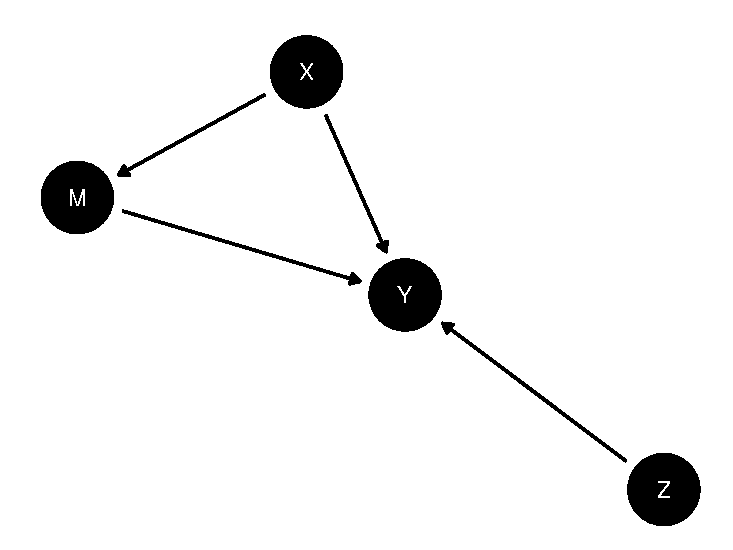
\includegraphics{paper_files/figure-pdf/unnamed-chunk-7-1.pdf}

}

\caption{A plotted model.}

\end{figure}

\begin{verbatim}
make_model("X -> M -> Y <- X; Z -> Y") |>
  plot(x_coord = 1:4,
       y_coord = c(1.5,2,1,2),
       title = "With options",
       textcol = "white",
       textsize = 3,
       shape = 18,
       nodecol = "grey",
       nodesize = 12) +
  theme(plot.background = element_rect(colour = "grey", fill=NA, linewidth=2))
\end{verbatim}

\begin{figure}[H]

{\centering 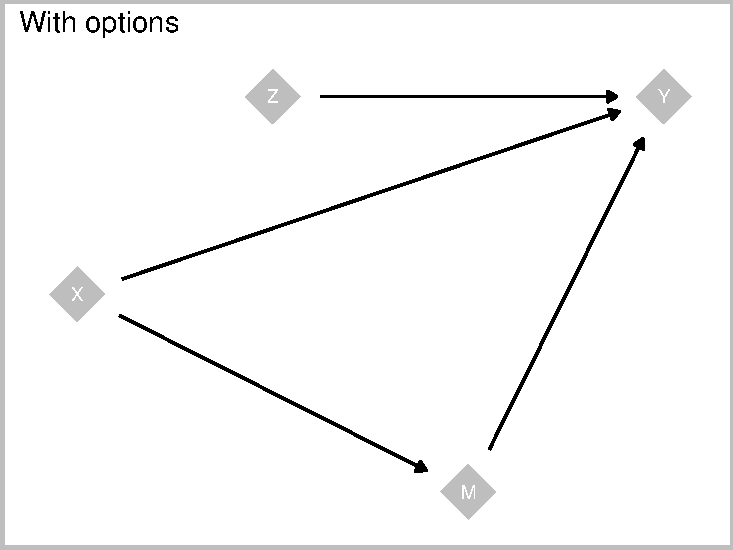
\includegraphics{paper_files/figure-pdf/unnamed-chunk-8-1.pdf}

}

\caption{A plotted model, showing options.}

\end{figure}

\hypertarget{model-characterization}{%
\subsection{Model characterization}\label{model-characterization}}

When a model is defined, a set of objects is generated. These are the
key quantities that are used for all inference. The table below
summarizes the core components of a model, providing a brief explanation
for each one.

The first element is a \texttt{statement} which defines how the nodes in
the model are related, specified by the user using dagitty syntax. The
second element, \texttt{dag}, is a data frame that outlines the
parent-child relationships within the model. \texttt{Nodes} is simply a
list of the node names in the model. Lastly, \texttt{parents\_df,} is a
table listing the nodes, indicating if they are root nodes, and showing
how many parents each node has.

The model includes additional elements, \texttt{nodal\_types,}
\texttt{parameters\_df,} and \texttt{causal\_types,} which we explain
later in detail .

\begin{longtable}[]{@{}
  >{\raggedright\arraybackslash}p{(\columnwidth - 2\tabcolsep) * \real{0.1462}}
  >{\raggedright\arraybackslash}p{(\columnwidth - 2\tabcolsep) * \real{0.8538}}@{}}
\toprule\noalign{}
\begin{minipage}[b]{\linewidth}\raggedright
Element
\end{minipage} & \begin{minipage}[b]{\linewidth}\raggedright
Description
\end{minipage} \\
\midrule\noalign{}
\endfirsthead
\toprule\noalign{}
\begin{minipage}[b]{\linewidth}\raggedright
Element
\end{minipage} & \begin{minipage}[b]{\linewidth}\raggedright
Description
\end{minipage} \\
\midrule\noalign{}
\endhead
\bottomrule\noalign{}
\endlastfoot
statement & A character string that describes directed causal relations
between variables in a causal model, where arrows denote that one node
is a potential cause of another. \\
dag & A data frame with columns `parent' and `children' indicating how
nodes relate to each other. \\
nodes & A list containing the nodes in the model. \\
parents\_df & A table listing nodes, whether they are root nodes or not,
and the number of parents they have. \\
nodal\_types & A list with the nodal types in the model. (See Nodal
Types Section) \\
parameters\_df & A data frame linking the model's parameters with the
nodal types of the model, as well as the family to which they belong.
(See Parameters dataframe Section) \\
causal\_types & A data frame listing causal types and the nodal types
that produce them. (See Causal Types Section) \\
P: parameter matrix & Should I include it? \\
\caption{Core Elements of a Causal Model}\tabularnewline
\end{longtable}

After updating a model, two additional components are attached to it:

\begin{itemize}
\item
  A posterior distribution of the parameters in the model, generated by
  stan. This distribution reflects the updated parameter values.
\item
  A list of objects, which we refer to as \texttt{stan\_objects}. The
  \texttt{stan\_objects} will, at a minimum, include the distribution of
  nodal types and the data used for updating the model
\end{itemize}

Optionally, users can choose whether to keep and append additional
elements to the \texttt{stan\_objects.} For instance, they can specify
whether to include \texttt{w}, which maps parameters to event
probabilities, as well as the `stanfit' object, the output generated by
stan

The table below summarizes the objects attached to the model after
updating.

\begin{longtable}[]{@{}
  >{\raggedright\arraybackslash}p{(\columnwidth - 2\tabcolsep) * \real{0.2312}}
  >{\raggedright\arraybackslash}p{(\columnwidth - 2\tabcolsep) * \real{0.7688}}@{}}
\toprule\noalign{}
\begin{minipage}[b]{\linewidth}\raggedright
Element
\end{minipage} & \begin{minipage}[b]{\linewidth}\raggedright
Description
\end{minipage} \\
\midrule\noalign{}
\endhead
\bottomrule\noalign{}
\endlastfoot
posterior\_distribution & The posterir distribution of the updated
parameters generated by stan. \\
stan\_objects & A list of objects, including, at a minimum,
\texttt{type\_distribution} and \texttt{data}. \\
data & The data used for updating the model, appended to
\texttt{stan\_objects.} \\
type\_distribution & The updated distribution of the nodal types,
appended to \texttt{stan\_objects.} \\
w & A mapping from parameters to event probabilities, optionally
appended to \texttt{stan\_objects.} \\
stan\_fit & The \texttt{stanfit} object generated by stan. This is
optionally appended to \texttt{stan\_objects.} \\
\end{longtable}

\hypertarget{parameters-dataframe}{%
\subsubsection{Parameters dataframe}\label{parameters-dataframe}}

When a model is created, \texttt{CausalQueries} attaches a ``parameters
dataframe'' which keeps track of model parameters, which belong together
in a family, and how they relate to causal types. This becomes
especially important for more complex models with confounding that might
involve more complicated mappings between parameters and nodal types. In
the case with no confounding the nodal types \emph{are} the parameters;
in cases with confounding you generally have more parameters than nodal
types.

For instance:

\begin{verbatim}
make_model("X->Y")$parameters_df |>
  kable()
\end{verbatim}

\begin{longtable}[]{@{}
  >{\raggedright\arraybackslash}p{(\columnwidth - 14\tabcolsep) * \real{0.1791}}
  >{\raggedright\arraybackslash}p{(\columnwidth - 14\tabcolsep) * \real{0.0746}}
  >{\raggedleft\arraybackslash}p{(\columnwidth - 14\tabcolsep) * \real{0.0597}}
  >{\raggedright\arraybackslash}p{(\columnwidth - 14\tabcolsep) * \real{0.1493}}
  >{\raggedright\arraybackslash}p{(\columnwidth - 14\tabcolsep) * \real{0.1642}}
  >{\raggedright\arraybackslash}p{(\columnwidth - 14\tabcolsep) * \real{0.0896}}
  >{\raggedleft\arraybackslash}p{(\columnwidth - 14\tabcolsep) * \real{0.1791}}
  >{\raggedleft\arraybackslash}p{(\columnwidth - 14\tabcolsep) * \real{0.1045}}@{}}
\toprule\noalign{}
\begin{minipage}[b]{\linewidth}\raggedright
param\_names
\end{minipage} & \begin{minipage}[b]{\linewidth}\raggedright
node
\end{minipage} & \begin{minipage}[b]{\linewidth}\raggedleft
gen
\end{minipage} & \begin{minipage}[b]{\linewidth}\raggedright
param\_set
\end{minipage} & \begin{minipage}[b]{\linewidth}\raggedright
nodal\_type
\end{minipage} & \begin{minipage}[b]{\linewidth}\raggedright
given
\end{minipage} & \begin{minipage}[b]{\linewidth}\raggedleft
param\_value
\end{minipage} & \begin{minipage}[b]{\linewidth}\raggedleft
priors
\end{minipage} \\
\midrule\noalign{}
\endhead
\bottomrule\noalign{}
\endlastfoot
X.0 & X & 1 & X & 0 & & 0.50 & 1 \\
X.1 & X & 1 & X & 1 & & 0.50 & 1 \\
Y.00 & Y & 2 & Y & 00 & & 0.25 & 1 \\
Y.10 & Y & 2 & Y & 10 & & 0.25 & 1 \\
Y.01 & Y & 2 & Y & 01 & & 0.25 & 1 \\
Y.11 & Y & 2 & Y & 11 & & 0.25 & 1 \\
\end{longtable}

Each row in the dataframe corresponds to a single parameter.

The columns of the parameters data frame are understood as follows:

\begin{itemize}
\tightlist
\item
  \texttt{param\_names} gives the name of the parameter, in shorthand.
  For instance the parameter
  \(\lambda^X_0 = \Pr(\theta^X = \theta^X_0)\) has \texttt{par\_name}
  \texttt{X.0}. See section @ref(notation) for a summary of notation.
\item
  \texttt{param\_value} gives the (possibly default) parameter values.
  These are probabilities.\\
\item
  \texttt{param\_set} indicates which parameters group together to form
  a simplex. The parameters in a set have parameter values that sum to
  1. In this example \(\lambda^X_0 + \lambda^X_1 = 1\).
\item
  \texttt{node} indicates the node associated with the parameter. For
  parameter \texttt{\textbackslash{}lambda\^{}X\_0} this is \(X\).
\item
  \texttt{nodal\_type} indicates the nodal types associated with the
  parameter.
\item
  \texttt{gen} indicates the place in the partial causal ordering
  (generation) of the node associated with the parameter
\item
  \texttt{priors} gives (possibly default) Dirichlet priors arguments
  for parameters in a set. Values of 1 (.5) for all parameters in a set
  implies uniform (Jeffrey's) priors over this set.
\end{itemize}

Below we will see examples where the parameter dataframe helps keep
track of parameters that are created when confounding is added to a
model.

\hypertarget{nodal-types}{%
\subsubsection{Nodal types}\label{nodal-types}}

Two units have the same \emph{nodal type} at node \(Y\), \(\theta^Y\),
if their outcome at \(Y\) responds in the same ways to parents of \(Y\).

A node with \(k\) parents has \(2^{2^k}\) nodal types. The reason is
that with \(k\) parents, there are \(2^k\) possible values of the
parents and so \(2^{2^k}\) ways to respond to these possible parental
values. As a convention we say that a node with no parents has two nodal
types (0 or 1).

When a model is created the full set of ``nodal types'' is identified.
These are stored in the model. The subscripts become very long and hard
to parse for more complex models so the model object also includes a
guide to interpreting nodal type values. You can see them like this.

\begin{verbatim}
make_model("X -> Y")$nodal_types
\end{verbatim}

\begin{verbatim}
$X
[1] "0" "1"

$Y
[1] "00" "10" "01" "11"

attr(,"interpret")
attr(,"interpret")$X
  node position display interpretation
1    X       NA      X0          X = 0
2    X       NA      X1          X = 1

attr(,"interpret")$Y
  node position display interpretation
1    Y        1   Y[*]*      Y | X = 0
2    Y        2   Y*[*]      Y | X = 1
\end{verbatim}

Note that we use \(\theta^j\) to indicate nodal types because for
qualitative analysis the nodal types are often the parameters of
interest.

LM: section on lookup types; \texttt{interpret\_type} EXAMPLE with maybe
2 parents

\hypertarget{causal-types}{%
\subsubsection{Causal types}\label{causal-types}}

Causal types are collections of nodal types. Two units are of the same
\emph{causal type} if they have the same nodal type at every node. For
example in a \(X \rightarrow M \rightarrow Y\) model,
\(\theta = (\theta^X_0, \theta^M_{01}, \theta^Y_{10})\) is a type that
has \(X=0\), \(M\) responds positively to \(X\), and \(Y\) responds
positively to \(M\).

When a model is created, the full set of causal types is identified.
These are stored in the model object:

\begin{verbatim}
make_model("A -> B")$causal_types
\end{verbatim}

\begin{verbatim}
       A  B
A0.B00 0 00
A1.B00 1 00
A0.B10 0 10
A1.B10 1 10
A0.B01 0 01
A1.B01 1 01
A0.B11 0 11
A1.B11 1 11
\end{verbatim}

A model with \(n_j\) nodal types at node \(j\) has \(\prod_jn_j\) causal
types. Thus the set of causal types can be large. In the model
\((X\rightarrow M \rightarrow Y \leftarrow X)\) there are
\(2\times 4\times 16 = 128\) causal types.

Knowledge of a causal type tells you what values a unit would take, on
all nodes, absent an intervention. For example for a model
\(X \rightarrow M \rightarrow Y\) a type
\(\theta = (\theta^X_0, \theta^M_{01}, \theta^Y_{10})\) would imply data
\((X=0, M=0, Y=1)\). (The converse of this, of course, is the key to
updating: observation of data \((X=0, M=0, Y=1)\) result in more weight
placed on \(\theta^X_0\), \(\theta^M_{01}\), and \(\theta^Y_{10})\).)

Till: Show how realise\_outcomes connects causal types with data types:
Show for something with a do operation and without a do operation; point
out causal types on left

\hypertarget{parameter-matrix}{%
\subsubsection{Parameter matrix}\label{parameter-matrix}}

The parameters dataframe keeps track of parameter values and priors for
parameters but it does not provide a mapping between parameters and the
probability of causal types.

The parameter matrix (\(P\) matrix) can be added to the model to provide
this mapping. The \(P\) matrix has a row for each parameter and a column
for each causal type. For instance:

\begin{verbatim}
make_model("X->Y") |> 
  get_parameter_matrix() |>
  kable()
\end{verbatim}

\begin{longtable}[]{@{}lrrrrrrrr@{}}
\toprule\noalign{}
& X0.Y00 & X1.Y00 & X0.Y10 & X1.Y10 & X0.Y01 & X1.Y01 & X0.Y11 &
X1.Y11 \\
\midrule\noalign{}
\endhead
\bottomrule\noalign{}
\endlastfoot
X.0 & 1 & 0 & 1 & 0 & 1 & 0 & 1 & 0 \\
X.1 & 0 & 1 & 0 & 1 & 0 & 1 & 0 & 1 \\
Y.00 & 1 & 1 & 0 & 0 & 0 & 0 & 0 & 0 \\
Y.10 & 0 & 0 & 1 & 1 & 0 & 0 & 0 & 0 \\
Y.01 & 0 & 0 & 0 & 0 & 1 & 1 & 0 & 0 \\
Y.11 & 0 & 0 & 0 & 0 & 0 & 0 & 1 & 1 \\
\end{longtable}

The probability of a causal type is given by the product of the
parameters values for parameters whose row in the \(P\) matrix contains
a 1.

Below we will see examples where the \(P\) matrix helps keep track of
parameters that are created when confounding is added to a model. CROSS
REFERENCE

To speed up different operations it is sometuimes useful to have P added
to the model:

\begin{itemize}
\tightlist
\item
  \texttt{set\_parameter\_matrix}\ldots{}
\end{itemize}

\hypertarget{tailoring-models}{%
\subsection{Tailoring models}\label{tailoring-models}}

\hypertarget{restrictions}{%
\subsubsection{Setting restrictions}\label{restrictions}}

TILL: READ THROUGH

When a model is defined, the complete set of possible causal relations
are worked out. This set can be very large.

Sometimes for theoretical or practical reasons it is useful to constrain
the set of types. In \texttt{CausalQueries} this is done at the level of
nodal types, with restrictions on causal types following from
restrictions on nodal types.

For instance to impose an assumption that \(Y\) is not decreasing in
\(X\) we generate a restricted model as follows:

\begin{verbatim}
model <- make_model("X->Y") |> set_restrictions("Y[X=1] < Y[X=0]")
\end{verbatim}

or:

\begin{verbatim}
model <- make_model("X->Y") |> set_restrictions(decreasing("X", "Y"))
\end{verbatim}

Viewing the resulting parameter matrix we see that both the set of
parameters and the set of causal types are now restricted:

\begin{verbatim}
get_parameter_matrix(model)
\end{verbatim}

\begin{verbatim}

Rows are parameters, grouped in parameter sets

Columns are causal types

Cell entries indicate whether a parameter probability is used
in the calculation of causal type probability

     X0.Y00 X1.Y00 X0.Y01 X1.Y01 X0.Y11 X1.Y11
X.0       1      0      1      0      1      0
X.1       0      1      0      1      0      1
Y.00      1      1      0      0      0      0
Y.01      0      0      1      1      0      0
Y.11      0      0      0      0      1      1

 
 param_set  (P)
 
\end{verbatim}

Here and in general, setting restrictions typically involves using
causal syntax; see Section @ref(syntax) for a guide the syntax used by
\texttt{CausalQueries}.

Note:

\begin{itemize}
\tightlist
\item
  Restrictions have to operate on nodal types: restrictions on
  \emph{levels} of endogenous nodes aren't allowed. This, for example,
  will fail:
  \texttt{make\_model("X-\textgreater{}Y")\ \textbar{}\textgreater{}\ set\_restrictions(statement\ =\ \ "(Y\ ==\ 1)")}.
  The reason is that it requests a correlated restriction on nodal types
  for \texttt{X} and \texttt{Y} which involves undeclared confounding.
\item
  Restrictions implicitly assume fixed values for \emph{all} parents of
  a node. For instance:
  \texttt{make\_model("A\ -\textgreater{}\ B\ \textless{}-\ C")\ \textbar{}\textgreater{}\ set\_restrictions("(B{[}C=1{]}==1)")}
  is interpreted as shorthand for the restriction
  \texttt{"B{[}C\ =\ 1,\ A\ =\ 0{]}==1\ \textbar{}\ B{[}C\ =\ 1,\ A\ =\ 1{]}==1"}.
\item
  To place restrictions on multiple nodes at the same time, provide
  these as a vector of restrictions. This is not permitted:
  \texttt{set\_restrictions("Y{[}X=1{]}==1\ \&\ X==1")}, since it
  requests correlated restrictions. This however is allowed:
  \texttt{set\_restrictions(c("Y{[}X=1{]}==1",\ "X==1"))}.\\
\item
  Use the \texttt{keep} argument to indicate whether nodal types should
  be dropped (default) or retained.
\item
  Restrictions can be set using nodal type labels.
\end{itemize}

\begin{verbatim}
make_model("S -> C -> Y <- R <- X; X -> C -> R") |>
  set_restrictions(labels = list(C = "1000", R = "0001", Y = "0001"), 
                   keep = TRUE)
\end{verbatim}

\begin{itemize}
\tightlist
\item
  Wild cards can be used in nodal type labels:
\end{itemize}

\begin{verbatim}
make_model("X->Y") |>
  set_restrictions(labels = list(Y = "Y?0"))
\end{verbatim}

\begin{itemize}
\tightlist
\item
  adding ``given'' for restrictions with models with confounding
\end{itemize}

\hypertarget{confounding}{%
\subsubsection{Allowing confounding}\label{confounding}}

(Unobserved) confounding between two nodes arises when the nodal types
for the nodes are not independently distributed.

In the \(X \rightarrow Y\) graph, for instance, there are 2 nodal types
for \(X\) and 4 for \(Y\). There are thus 8 joint nodal types (or causal
types):

\begin{longtable}[]{@{}
  >{\centering\arraybackslash}p{(\columnwidth - 8\tabcolsep) * \real{0.0517}}
  >{\centering\arraybackslash}p{(\columnwidth - 8\tabcolsep) * \real{0.0690}}
  >{\centering\arraybackslash}p{(\columnwidth - 8\tabcolsep) * \real{0.3448}}
  >{\raggedright\arraybackslash}p{(\columnwidth - 8\tabcolsep) * \real{0.3448}}
  >{\raggedright\arraybackslash}p{(\columnwidth - 8\tabcolsep) * \real{0.1897}}@{}}
\toprule\noalign{}
\begin{minipage}[b]{\linewidth}\centering
\end{minipage} & \begin{minipage}[b]{\linewidth}\centering
\end{minipage} & \begin{minipage}[b]{\linewidth}\centering
\(\theta^X\)
\end{minipage} & \begin{minipage}[b]{\linewidth}\raggedright
\end{minipage} & \begin{minipage}[b]{\linewidth}\raggedright
\end{minipage} \\
\midrule\noalign{}
\endhead
\bottomrule\noalign{}
\endlastfoot
& & 0 & 1 & Sum \\
\(\theta^Y\) & 00 & \(\Pr(\theta^X_0, \theta^Y_{00})\) &
\(\Pr(\theta^X_1, \theta^Y_{00})\) & \(\Pr(\theta^Y_{00})\) \\
& 10 & \(\Pr(\theta^X_0, \theta^Y_{10})\) &
\(\Pr(\theta^X_1, \theta^Y_{10})\) & \(\Pr(\theta^Y_{10})\) \\
& 01 & \(\Pr(\theta^X_0, \theta^Y_{01})\) &
\(\Pr(\theta^X_1, \theta^Y_{01})\) & \(\Pr(\theta^Y_{01})\) \\
& 11 & \(\Pr(\theta^X_0, \theta^Y_{11})\) &
\(\Pr(\theta^X_1, \theta^Y_{11})\) & \(\Pr(\theta^Y_{11})\) \\
& Sum & \(\Pr(\theta^X_0)\) & \(\Pr(\theta^X_1)\) & 1 \\
\end{longtable}

This table has 8 interior elements and so an unconstrained joint
distribution would have 7 degrees of freedom. A no confounding
assumption means that \(\Pr(\theta^X | \theta^Y) = \Pr(\theta^X)\), or
\(\Pr(\theta^X, \theta^Y) = \Pr(\theta^X)\Pr(\theta^Y)\). In this case
we just put a distribution on the marginals and there would be 3 degrees
of freedom for \(Y\) and 1 for \(X\), totaling \(4\) rather than 7.

\begin{verbatim}
confounded <- make_model("X->Y ; X <-> Y")

confounded$parameters_df |> kable()
\end{verbatim}

\begin{longtable}[]{@{}
  >{\raggedright\arraybackslash}p{(\columnwidth - 14\tabcolsep) * \real{0.1791}}
  >{\raggedright\arraybackslash}p{(\columnwidth - 14\tabcolsep) * \real{0.0746}}
  >{\raggedleft\arraybackslash}p{(\columnwidth - 14\tabcolsep) * \real{0.0597}}
  >{\raggedright\arraybackslash}p{(\columnwidth - 14\tabcolsep) * \real{0.1493}}
  >{\raggedright\arraybackslash}p{(\columnwidth - 14\tabcolsep) * \real{0.1642}}
  >{\raggedright\arraybackslash}p{(\columnwidth - 14\tabcolsep) * \real{0.0896}}
  >{\raggedleft\arraybackslash}p{(\columnwidth - 14\tabcolsep) * \real{0.1791}}
  >{\raggedleft\arraybackslash}p{(\columnwidth - 14\tabcolsep) * \real{0.1045}}@{}}
\toprule\noalign{}
\begin{minipage}[b]{\linewidth}\raggedright
param\_names
\end{minipage} & \begin{minipage}[b]{\linewidth}\raggedright
node
\end{minipage} & \begin{minipage}[b]{\linewidth}\raggedleft
gen
\end{minipage} & \begin{minipage}[b]{\linewidth}\raggedright
param\_set
\end{minipage} & \begin{minipage}[b]{\linewidth}\raggedright
nodal\_type
\end{minipage} & \begin{minipage}[b]{\linewidth}\raggedright
given
\end{minipage} & \begin{minipage}[b]{\linewidth}\raggedleft
param\_value
\end{minipage} & \begin{minipage}[b]{\linewidth}\raggedleft
priors
\end{minipage} \\
\midrule\noalign{}
\endhead
\bottomrule\noalign{}
\endlastfoot
X.0 & X & 1 & X & 0 & & 0.50 & 1 \\
X.1 & X & 1 & X & 1 & & 0.50 & 1 \\
Y.00\_X.0 & Y & 2 & Y.X.0 & 00 & X.0 & 0.25 & 1 \\
Y.10\_X.0 & Y & 2 & Y.X.0 & 10 & X.0 & 0.25 & 1 \\
Y.01\_X.0 & Y & 2 & Y.X.0 & 01 & X.0 & 0.25 & 1 \\
Y.11\_X.0 & Y & 2 & Y.X.0 & 11 & X.0 & 0.25 & 1 \\
Y.00\_X.1 & Y & 2 & Y.X.1 & 00 & X.1 & 0.25 & 1 \\
Y.10\_X.1 & Y & 2 & Y.X.1 & 10 & X.1 & 0.25 & 1 \\
Y.01\_X.1 & Y & 2 & Y.X.1 & 01 & X.1 & 0.25 & 1 \\
Y.11\_X.1 & Y & 2 & Y.X.1 & 11 & X.1 & 0.25 & 1 \\
\end{longtable}

We see here that there are now two parameter families for parameters
associated with the node \(Y\). Each family captures the conditional
distribution of \(Y\)'s nodal types, given \(X\). For instance the
parameter \texttt{Y01\_X.1} can be interpreted as
\(\Pr(\theta^Y = \theta^Y_{01} | X=1)\).

To see exactly how the parameters map to causal types we can view the
parameter matrix:

\begin{verbatim}
get_parameter_matrix(confounded) |> kable()
\end{verbatim}

\begin{longtable}[]{@{}
  >{\raggedright\arraybackslash}p{(\columnwidth - 16\tabcolsep) * \real{0.1385}}
  >{\raggedleft\arraybackslash}p{(\columnwidth - 16\tabcolsep) * \real{0.1077}}
  >{\raggedleft\arraybackslash}p{(\columnwidth - 16\tabcolsep) * \real{0.1077}}
  >{\raggedleft\arraybackslash}p{(\columnwidth - 16\tabcolsep) * \real{0.1077}}
  >{\raggedleft\arraybackslash}p{(\columnwidth - 16\tabcolsep) * \real{0.1077}}
  >{\raggedleft\arraybackslash}p{(\columnwidth - 16\tabcolsep) * \real{0.1077}}
  >{\raggedleft\arraybackslash}p{(\columnwidth - 16\tabcolsep) * \real{0.1077}}
  >{\raggedleft\arraybackslash}p{(\columnwidth - 16\tabcolsep) * \real{0.1077}}
  >{\raggedleft\arraybackslash}p{(\columnwidth - 16\tabcolsep) * \real{0.1077}}@{}}
\toprule\noalign{}
\begin{minipage}[b]{\linewidth}\raggedright
\end{minipage} & \begin{minipage}[b]{\linewidth}\raggedleft
X0.Y00
\end{minipage} & \begin{minipage}[b]{\linewidth}\raggedleft
X1.Y00
\end{minipage} & \begin{minipage}[b]{\linewidth}\raggedleft
X0.Y10
\end{minipage} & \begin{minipage}[b]{\linewidth}\raggedleft
X1.Y10
\end{minipage} & \begin{minipage}[b]{\linewidth}\raggedleft
X0.Y01
\end{minipage} & \begin{minipage}[b]{\linewidth}\raggedleft
X1.Y01
\end{minipage} & \begin{minipage}[b]{\linewidth}\raggedleft
X0.Y11
\end{minipage} & \begin{minipage}[b]{\linewidth}\raggedleft
X1.Y11
\end{minipage} \\
\midrule\noalign{}
\endhead
\bottomrule\noalign{}
\endlastfoot
X.0 & 1 & 0 & 1 & 0 & 1 & 0 & 1 & 0 \\
X.1 & 0 & 1 & 0 & 1 & 0 & 1 & 0 & 1 \\
Y.00\_X.0 & 1 & 0 & 0 & 0 & 0 & 0 & 0 & 0 \\
Y.10\_X.0 & 0 & 0 & 1 & 0 & 0 & 0 & 0 & 0 \\
Y.01\_X.0 & 0 & 0 & 0 & 0 & 1 & 0 & 0 & 0 \\
Y.11\_X.0 & 0 & 0 & 0 & 0 & 0 & 0 & 1 & 0 \\
Y.00\_X.1 & 0 & 1 & 0 & 0 & 0 & 0 & 0 & 0 \\
Y.10\_X.1 & 0 & 0 & 0 & 1 & 0 & 0 & 0 & 0 \\
Y.01\_X.1 & 0 & 0 & 0 & 0 & 0 & 1 & 0 & 0 \\
Y.11\_X.1 & 0 & 0 & 0 & 0 & 0 & 0 & 0 & 1 \\
\end{longtable}

Importantly, the \(P\) matrix works as before, despite confounding. We
can assess the probability of causal types by multiplying the
probabilities of the constituent parameters.

\begin{itemize}
\tightlist
\item
  Unlike nodal restrictions, a confounding relation can involve multiple
  nodal types simultaneously. For instance
  \texttt{make\_model("X\ -\textgreater{}\ M\ -\textgreater{}\ Y")\ \textbar{}\textgreater{}\ set\_confound(list(X\ =\ "Y{[}X=1{]}\ \textgreater{}\ Y{[}X=0{]}"))}
  allows for a parameter that renders \(X\) more or less likely
  depending on whether \(X\) has a positive effect on \(Y\) whether it
  runs through a positive or a negative effect on \(M\).
\item
  The parameters needed to capture confounding relations depend on the
  direction of causal arrows. For example compare:

  \begin{itemize}
  \tightlist
  \item
    \texttt{make\_model("A\ -\textgreater{}\ W\ \textless{}-\ B\ ;\ A\ \textless{}-\textgreater{}\ W;\ B\ \textless{}-\textgreater{}\ W")\$parameters\_df\ \textbar{}\textgreater{}\ dim}
    In this case we can decompose shocks on \(A, B, W\) via:
    \(\Pr(\theta^A, \theta^B, \theta^W) = \Pr(\theta^W | \theta^A, \theta^A)\Pr(\theta^A)\Pr(\theta^B)\),
    and we have 68 parameters.
  \item
    \texttt{make\_model("A\ \textless{}-\ W\ -\textgreater{}\ B\ ;\ A\ \textless{}-\textgreater{}\ W;\ B\ \textless{}-\textgreater{}\ W")\$parameters\_df\ \textbar{}\textgreater{}\ dim}
    In this case we have
    \(\Pr(\theta^A, \theta^B, \theta^W) = \Pr(\theta^A | \theta^W)\Pr(\theta^B|\theta^W)\Pr(\theta^W)\)
    and just has just 18 parameters.
  \end{itemize}
\end{itemize}

\begin{verbatim}
make_model("A <- X -> B; A <-> X; B <-> X") |> 
  plot()
\end{verbatim}

\begin{figure}[H]

{\centering 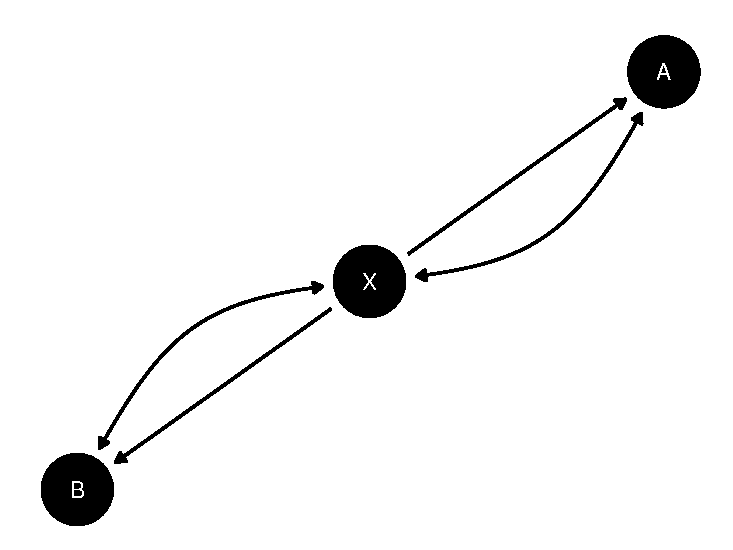
\includegraphics{paper_files/figure-pdf/unnamed-chunk-20-1.pdf}

}

\end{figure}

\hypertarget{priors}{%
\subsubsection{Setting Priors}\label{priors}}

Priors on model parameters can be added to the parameters dataframe. The
priors are interpreted as alpha arguments for a Dirichlet distribution.
They can be seen using \texttt{get\_priors}.

MH: TEXT ON DIRICHLET

\begin{verbatim}
make_model("X->Y") |> get_priors()
\end{verbatim}

\begin{verbatim}
 X.0  X.1 Y.00 Y.10 Y.01 Y.11 
   1    1    1    1    1    1 
\end{verbatim}

Here the priors have not been specified and so they default to 1, which
corresponds to uniform priors.

Alternatively you could set jeffreys priors like this:

\begin{verbatim}
make_model("X->Y") |> 
  set_priors(distribution = "jeffreys") |> 
  get_priors()
\end{verbatim}

\begin{verbatim}
No specific parameters to alter values for specified. Altering all parameters.
\end{verbatim}

\begin{verbatim}
 X.0  X.1 Y.00 Y.10 Y.01 Y.11 
 0.5  0.5  0.5  0.5  0.5  0.5 
\end{verbatim}

Custom priors are most simply specified by being added as a vector of
numbers using \texttt{set\_priors}. For instance:

\begin{verbatim}
make_model("X->Y") |> 
  set_priors(1:6) |> 
  get_priors()
\end{verbatim}

\begin{verbatim}
 X.0  X.1 Y.00 Y.10 Y.01 Y.11 
   1    2    3    4    5    6 
\end{verbatim}

The priors here should be interpreted as indicating:

\begin{itemize}
\tightlist
\item
  \(\alpha_X = (1,2)\), which implies a distribution over
  \((\lambda^X_0, \lambda^X_1)\) centered on \((1/3, 2/3)\).
\item
  \(\alpha_Y = (3,4,5,6)\), which implies a distribution over
  \((\lambda^Y_{00}, \lambda^Y_{10}, \lambda^Y_{01} \lambda^Y_{11})\)
  centered on \((3/18, 4/18, 5/18, 6/18)\).
\end{itemize}

For larger models it can be hard to provide priors as a vector of
numbers and so \texttt{set\_priors} can allow for more targeted
modifications of the parameter vector. For instance:

\begin{verbatim}
make_model("X->Y") |>
  set_priors(statement = "Y[X=1] > Y[X=0]", alphas = 3) |>
  get_priors()
\end{verbatim}

\begin{verbatim}
 X.0  X.1 Y.00 Y.10 Y.01 Y.11 
   1    1    1    1    3    1 
\end{verbatim}

As setting priors simply requires mapping alpha values to parameters;
the process boils down to selecting rows of the \texttt{parmeters\_df}
dataframe, at which to alter values. When specifying a causal statement
as above, CausalQueries internally identifies nodal types that are
consistent with the statement, which in turn identify parameters to
alter priors for. Note that there is nothing particularly unique about
setting priors via causal syntax, as it is simply an abstract way of
specifying how to subset the \texttt{parameters\_df} dataframe. To wit;
we can achieve the same result as above by specifying:

\begin{verbatim}
make_model("X->Y") |>
  set_priors(nodal_type = "01", alphas = 3) |>
  get_priors()
\end{verbatim}

\begin{verbatim}
 X.0  X.1 Y.00 Y.10 Y.01 Y.11 
   1    1    1    1    3    1 
\end{verbatim}

or even:

\begin{verbatim}
make_model("X->Y") |>
  set_priors(param_names = "Y.01", alphas = 3) |>
  get_priors()
\end{verbatim}

\begin{verbatim}
 X.0  X.1 Y.00 Y.10 Y.01 Y.11 
   1    1    1    1    3    1 
\end{verbatim}

\texttt{set\_priors} allows for the specification of any non-redundant
combination of arguments on the \texttt{param\_names}, \texttt{node},
\texttt{nodal\_type}, \texttt{param\_set} and \texttt{given} columns of
\texttt{parameters\_df} to uniquely identify parameters to set priors
on. Alternatively a fully formed subsetting statement may be supplied to
\texttt{alter\_at}. As all these arguments get mapped to the parameters
the identify internally they may be used interchangeably.

\begin{verbatim}
make_model("X-> M -> Y; X <-> Y") |>
  set_priors(node = "Y", nodal_type = c("01","11"), given = "X.1", alphas = c(3,2)) |>
  get_priors()
\end{verbatim}

\begin{verbatim}
     X.0      X.1     M.00     M.10     M.01     M.11 Y.00_X.0 Y.10_X.0 
       1        1        1        1        1        1        1        1 
Y.01_X.0 Y.11_X.0 Y.00_X.1 Y.10_X.1 Y.01_X.1 Y.11_X.1 
       1        1        1        1        3        2 
\end{verbatim}

\begin{verbatim}
make_model("X-> M -> Y; X <-> Y") |>
  set_priors(alter_at = "node == 'Y' & nodal_type %in% c('01','11') & given == 'X.1'", alphas = c(3,2)) |>
  get_priors()
\end{verbatim}

\begin{verbatim}
     X.0      X.1     M.00     M.10     M.01     M.11 Y.00_X.0 Y.10_X.0 
       1        1        1        1        1        1        1        1 
Y.01_X.0 Y.11_X.0 Y.00_X.1 Y.10_X.1 Y.01_X.1 Y.11_X.1 
       1        1        1        1        3        2 
\end{verbatim}

It should be noted that while highly targeted prior setting is
convenient and flexible; it should be done with caution. Setting priors
on specific parameters in complex models; especially models involving
confounding, may strongly affect inferences in intractable ways.

See \texttt{?set\_priors} and \texttt{?make\_priors} for many examples.

We note that flat priors over nodal types does not necessarily translate
into flat priors over queries. ``Flat'' priors over parameters in a
parameter family put equal weight on each nodal type, but this in turn
can translate into strong assumptions on causal quantities of interest.

For instance in an \(X \rightarrow Y\) model model in which negative
effects are ruled out, the average causal effect implied by ``flat''
priors is \(1/3\). This can be seen by querying the model:

\begin{verbatim}
make_model("X -> Y") |>
  set_restrictions(decreasing("X", "Y")) |>
  query_model("Y[X=1] - Y[X=0]", n_draws = 10000) |>
  kable(digits = 2)
\end{verbatim}

\begin{longtable}[]{@{}
  >{\raggedright\arraybackslash}p{(\columnwidth - 14\tabcolsep) * \real{0.1951}}
  >{\raggedright\arraybackslash}p{(\columnwidth - 14\tabcolsep) * \real{0.0732}}
  >{\raggedright\arraybackslash}p{(\columnwidth - 14\tabcolsep) * \real{0.1341}}
  >{\raggedright\arraybackslash}p{(\columnwidth - 14\tabcolsep) * \real{0.1341}}
  >{\raggedleft\arraybackslash}p{(\columnwidth - 14\tabcolsep) * \real{0.0610}}
  >{\raggedleft\arraybackslash}p{(\columnwidth - 14\tabcolsep) * \real{0.0366}}
  >{\raggedleft\arraybackslash}p{(\columnwidth - 14\tabcolsep) * \real{0.1707}}
  >{\raggedleft\arraybackslash}p{(\columnwidth - 14\tabcolsep) * \real{0.1951}}@{}}
\toprule\noalign{}
\begin{minipage}[b]{\linewidth}\raggedright
query
\end{minipage} & \begin{minipage}[b]{\linewidth}\raggedright
given
\end{minipage} & \begin{minipage}[b]{\linewidth}\raggedright
using
\end{minipage} & \begin{minipage}[b]{\linewidth}\raggedright
case\_level
\end{minipage} & \begin{minipage}[b]{\linewidth}\raggedleft
mean
\end{minipage} & \begin{minipage}[b]{\linewidth}\raggedleft
sd
\end{minipage} & \begin{minipage}[b]{\linewidth}\raggedleft
cred.low.2.5\%
\end{minipage} & \begin{minipage}[b]{\linewidth}\raggedleft
cred.high.97.5\%
\end{minipage} \\
\midrule\noalign{}
\endhead
\bottomrule\noalign{}
\endlastfoot
Y{[}X=1{]} - Y{[}X=0{]} & - & parameters & FALSE & 0.33 & NA & 0.33 &
0.33 \\
\end{longtable}

More subtly the \emph{structure} of a model, coupled with flat priors,
has substantive importance for priors on causal quantities. For instance
with flat priors, priors on the probability that \(X\) has a positive
effect on \(Y\) in the model \(X \rightarrow Y\) is centered on \(1/4\).
But priors on the probability that \(X\) has a positive effect on \(Y\)
in the model \(X \rightarrow M \rightarrow Y\) is centered on \(1/8\).

Again, you can use \texttt{query\_model} to figure out what flat (or
other) priors over parameters imply for priors over causal quantities:

\begin{verbatim}
make_model("X -> Y") |>
  query_model("Y[X=1] > Y[X=0]", n_draws = 10000) |>
  kable()
\end{verbatim}

\begin{longtable}[]{@{}
  >{\raggedright\arraybackslash}p{(\columnwidth - 14\tabcolsep) * \real{0.1951}}
  >{\raggedright\arraybackslash}p{(\columnwidth - 14\tabcolsep) * \real{0.0732}}
  >{\raggedright\arraybackslash}p{(\columnwidth - 14\tabcolsep) * \real{0.1341}}
  >{\raggedright\arraybackslash}p{(\columnwidth - 14\tabcolsep) * \real{0.1341}}
  >{\raggedleft\arraybackslash}p{(\columnwidth - 14\tabcolsep) * \real{0.0610}}
  >{\raggedleft\arraybackslash}p{(\columnwidth - 14\tabcolsep) * \real{0.0366}}
  >{\raggedleft\arraybackslash}p{(\columnwidth - 14\tabcolsep) * \real{0.1707}}
  >{\raggedleft\arraybackslash}p{(\columnwidth - 14\tabcolsep) * \real{0.1951}}@{}}
\toprule\noalign{}
\begin{minipage}[b]{\linewidth}\raggedright
query
\end{minipage} & \begin{minipage}[b]{\linewidth}\raggedright
given
\end{minipage} & \begin{minipage}[b]{\linewidth}\raggedright
using
\end{minipage} & \begin{minipage}[b]{\linewidth}\raggedright
case\_level
\end{minipage} & \begin{minipage}[b]{\linewidth}\raggedleft
mean
\end{minipage} & \begin{minipage}[b]{\linewidth}\raggedleft
sd
\end{minipage} & \begin{minipage}[b]{\linewidth}\raggedleft
cred.low.2.5\%
\end{minipage} & \begin{minipage}[b]{\linewidth}\raggedleft
cred.high.97.5\%
\end{minipage} \\
\midrule\noalign{}
\endhead
\bottomrule\noalign{}
\endlastfoot
Y{[}X=1{]} \textgreater{} Y{[}X=0{]} & - & parameters & FALSE & 0.25 &
NA & 0.25 & 0.25 \\
\end{longtable}

\begin{verbatim}
make_model("X -> M -> Y") |>
  query_model("Y[X=1] > Y[X=0]", n_draws = 10000) |>
  kable()
\end{verbatim}

\begin{longtable}[]{@{}
  >{\raggedright\arraybackslash}p{(\columnwidth - 14\tabcolsep) * \real{0.1928}}
  >{\raggedright\arraybackslash}p{(\columnwidth - 14\tabcolsep) * \real{0.0723}}
  >{\raggedright\arraybackslash}p{(\columnwidth - 14\tabcolsep) * \real{0.1325}}
  >{\raggedright\arraybackslash}p{(\columnwidth - 14\tabcolsep) * \real{0.1325}}
  >{\raggedleft\arraybackslash}p{(\columnwidth - 14\tabcolsep) * \real{0.0723}}
  >{\raggedleft\arraybackslash}p{(\columnwidth - 14\tabcolsep) * \real{0.0361}}
  >{\raggedleft\arraybackslash}p{(\columnwidth - 14\tabcolsep) * \real{0.1687}}
  >{\raggedleft\arraybackslash}p{(\columnwidth - 14\tabcolsep) * \real{0.1928}}@{}}
\toprule\noalign{}
\begin{minipage}[b]{\linewidth}\raggedright
query
\end{minipage} & \begin{minipage}[b]{\linewidth}\raggedright
given
\end{minipage} & \begin{minipage}[b]{\linewidth}\raggedright
using
\end{minipage} & \begin{minipage}[b]{\linewidth}\raggedright
case\_level
\end{minipage} & \begin{minipage}[b]{\linewidth}\raggedleft
mean
\end{minipage} & \begin{minipage}[b]{\linewidth}\raggedleft
sd
\end{minipage} & \begin{minipage}[b]{\linewidth}\raggedleft
cred.low.2.5\%
\end{minipage} & \begin{minipage}[b]{\linewidth}\raggedleft
cred.high.97.5\%
\end{minipage} \\
\midrule\noalign{}
\endhead
\bottomrule\noalign{}
\endlastfoot
Y{[}X=1{]} \textgreater{} Y{[}X=0{]} & - & parameters & FALSE & 0.125 &
NA & 0.125 & 0.125 \\
\end{longtable}

Caution regarding priors is particularly important when models are not
identified, as is the case for many of the models considered here. In
such cases, for some quantities, the marginal posterior distribution can
be the same as the marginal prior distribution
\citep{poirier1998revising}.

The key point here is to make sure you do not fall into a trap of
thinking that ``uninformative'' priors make no commitments regarding the
values of causal quantities of interest. They do, and the implications
of flat priors for causal quantities can depend on the structure of the
model. Moreover for some inferences from causal models the priors can
matter a lot even if you have a lot of data. In such cases it can be
helpful to know what priors on parameters imply for priors on causal
quantities of interest (by using \texttt{query\_model}) and to assess
how much conclusions depend on priors (by comparing results across
models that vary in their priors).

\hypertarget{parameters}{%
\subsubsection{Setting Parameters}\label{parameters}}

MH: POINT OUT FOLLOWING SAME LOGIC AS LASTS SECTION parameters rather
than alphas as arguments

By default, models have a vector of parameter values included in the
\texttt{parameters\_df} dataframe. These are useful for generating data,
or for situations, such as process tracing, when one wants to make
inferences about causal types (\(\theta\)), given case level data, under
the assumption that the model is known.

Consider the causal model below. It has two parameter sets, X and Y,
with six nodal types, two corresponding to X and four corresponding to
Y. The key feature of the parameters is that they must sum to 1 within
each parameter set.

\begin{verbatim}
make_model("X->Y") |> 
  get_parameters()
\end{verbatim}

\begin{verbatim}
 X.0  X.1 Y.00 Y.10 Y.01 Y.11 
0.50 0.50 0.25 0.25 0.25 0.25 
\end{verbatim}

Setting parameters can be done using a similar syntax as
\texttt{set\_priors}. The main difference is that when a given value is
altered the entire set must still always sum to 1. The example below
illustrates a change in the value of the parameter \(Y\) in the case it
is increasing in \(X\). Here nodal type \texttt{Y.Y01} is set to be .5,
while the other nodal types of this parameter set were renormalized so
that the parameters in the set still sum to one.

\begin{verbatim}
make_model("X->Y") |>
  set_parameters(statement = "Y[X=1] > Y[X=0]", parameters = .5) |>
  get_parameters()
\end{verbatim}

\begin{verbatim}
      X.0       X.1      Y.00      Y.10      Y.01      Y.11 
0.5000000 0.5000000 0.1666667 0.1666667 0.5000000 0.1666667 
\end{verbatim}

\hypertarget{drawing-and-manipulating-data}{%
\subsection{Drawing and manipulating
data}\label{drawing-and-manipulating-data}}

MH MAKE SENSE OF THIS HERE

\begin{verbatim}
model |> make_data(n = 5) |> kable()
\end{verbatim}

\begin{longtable}[]{@{}rr@{}}
\toprule\noalign{}
X & Y \\
\midrule\noalign{}
\endhead
\bottomrule\noalign{}
\endlastfoot
0 & 0 \\
0 & 0 \\
1 & 0 \\
1 & 1 \\
1 & 1 \\
\end{longtable}

LONG AND COMPACT FORMS

\hypertarget{updating-models}{%
\section{Updating models}\label{updating-models}}

The approach used by the \texttt{CausalQueries} package to updating
parameter values given observed data uses \texttt{stan} and involves the
following elements:

\begin{itemize}
\tightlist
\item
  Dirichlet priors over parameters, \(\lambda\) (which, in cases without
  confounding, correspond to nodal types)
\item
  A mapping from parameters to event probabilities, \(w\)
\item
  A likelihood function that assumes events are distributed according to
  a multinomial distribution given event probabilities.
\end{itemize}

We provide further details below.

\hypertarget{data-for-stan}{%
\subsection{Data for stan}\label{data-for-stan}}

GS: general edit to this section

We use a generic \texttt{stan} model that works for all binary causal
models. Rather than writing a new \texttt{stan} model for each causal
model we send \texttt{stan} details of each particular causal model as
data inputs.

In particular we provide a set of matrices that \texttt{stan} tailor
itself to particular models: the parameter matrix (\(P\) ) tells
\texttt{stan} how many parameters there are, and how they map into
causal types; an ambiguity matrix \(A\) tells \texttt{stan} how causal
types map into data types; and an event matrix \(E\) relates data types
into patterns of observed data (in cases where there are incomplete
observations).

The internal function \texttt{prep\_stan\_data} prepares data for
\texttt{stan}. You generally don't need to use this manually, but we
show here a sample of what it produces as input for \texttt{stan}.

Note that NAs are interpreted as data not having been sought. So in this
case the interpretation is that there are two data strategies: data on
\(Y\) and \(X\) was sought in three cases; data on \(Y\) only was sought
in just one case.

\hypertarget{how-the-stan-model-works}{%
\subsection{How the stan model works}\label{how-the-stan-model-works}}

THIS DISCUSSION IS OUT OF DATE:

The \texttt{stan} model works as follows:

MH: ADD DISCUSSION OF parmap;

\begin{itemize}
\item
  We are interested in ``sets'' of parameters. For example in the
  \(X \rightarrow Y\) model we have two parameter sets
  (\texttt{param\_sets}). The first is
  \(\lambda^X \in \{\lambda^X_0, \lambda^X_1\}\) whose elements give the
  probability that \(X\) is 0 or 1. These two probabilities sum to one.
  The second parameter set is
  \(\lambda^Y \in \{\lambda^Y_{00}, \lambda^Y_{10}, \lambda^Y_{01} \lambda^Y_{11}\}\).
  These are also probabilities and their values sum to one. Note in all
  that we have 6 parameters but just 1 + 3 = 4 degrees of freedom.
\item
  We would like to express priors over these parameters using multiple
  Dirichlet distributions (two in this case). In practice because we are
  dealing with multiple simplices of varying length, it is easier to
  express priors over gamma distributions with a unit scale parameter
  and shape parameter corresponding to the Dirichlet priors, \(\alpha\).
  We make use of the fact that \(\lambda^X_0 \sim Gamma(\alpha^X_0,1)\)
  and \(\lambda^X_1 \sim Gamma(\alpha^X_1,1)\) then
  \(\frac{1}{\lambda^X_0 +\lambda^X_1}(\lambda^X_0, \lambda^X_1) \sim Dirichlet(\alpha^X_0, \alpha^X_1)\).
  For a discussion of implementation of this approach in \texttt{stan}
  see https://discourse.mc-stan.org/t/ragged-array-of-simplexes/1382.
\item
  For any candidate parameter vector \(\lambda\) we calculate the
  probability of \emph{causal} types (\texttt{prob\_of\_types}) by
  taking, for each type \(i\), the product of the probabilities of all
  parameters (\(\lambda_j\)) that appear in column \(i\) of the
  parameter matrix \(P\). Thus the probability of a \((X_0,Y_{00})\)
  case is just \(\lambda^X_0 \times \lambda^Y_{00}\). The
  implementations in \texttt{stan} uses
  \texttt{prob\_of\_types\_{[}i{]}}
  \(= \prod_j \left(P_{j,i} \lambda_j + (1-P_{j,i})\right)\): this
  multiplies the probability of all parameters involved in the causal
  type (and substitutes 1s for parameters that are not). (\texttt{P} and
  \texttt{not\_P} (1-\(P\)) are provided as data to \texttt{stan}).
\item
  The probability of data types, \texttt{w}, is given by summing up the
  probabilities of all causal types that produce a given data type. For
  example, the probability of a \(X=0,Y=0\) case, \(w_{00}\) is
  \(\lambda^X_0\times \lambda^Y_{00} + \lambda^X_0\times \lambda^Y_{01}\).
  The ambiguity matrix \(A\) is provided to \texttt{stan} to indicate
  which probabilities need to be summed.
\item
  In the case of incomplete data we first identify the set of ``data
  strategies'', where a collection of a data strategy might be of the
  form ``gather data on \(X\) and \(M\), but not \(Y\), for \(n_1\)
  cases and gather data on \(X\) and \(Y\), but not \(M\), for \(n_2\)
  cases. The probability of an observed event, within a data strategy,
  is given by summing the probabilities of the types that could give
  rise to the incomplete data. For example \(X\) is observed, but \(Y\)
  is not, then the probability of \(X=0, Y = \text{NA}\) is
  \(w_{00} +w_{01}\). The matrix \(E\) is passed to \texttt{stan} to
  figure out which event probabilities need to be combined for events
  with missing data.
\item
  The probability of a dataset is then given by a multinomial
  distribution with these event probabilities (or, in the case of
  incomplete data, the product of multinomials, one for each data
  strategy).
\end{itemize}

GS: TO CHECK THE PATHS FUNCTIONALITY

\hypertarget{implementation}{%
\subsection{Implementation}\label{implementation}}

To update a CausalQueries model with data use:

\begin{verbatim}
update_model(model, data)
\end{verbatim}

where the data argument is a dataset containing some or all of the nodes
in the model.

As \texttt{update\_model()} calls \texttt{rstan::sampling} one can pass
along all arguments in \texttt{...} to \texttt{rstan::sampling}. For
instance:

\begin{itemize}
\tightlist
\item
  \texttt{iter} sets the number of iterations and ultimately the number
  of draws in the posterior
\item
  \texttt{chains} sets the number of chains; doing multiple chains in
  parallel speeds things up
\end{itemize}

If you have multiple cores you can do parallel processing by including
this line before running \texttt{CausalQueries}:

\begin{verbatim}
options(mc.cores = parallel::detectCores())
\end{verbatim}

Additionally parallelizing across models or data while running MCMC
chains in parallel can be achieved by setting up a nested parallel
process. With 8 cores one can run 2 updating processes with 3 parallel
chains each simultaneously. More generally the number of parallel
processes at the upper level of the nested parallel structure are given
by \texttt{floor(cores/(chains\ +\ 1))}.

\begin{verbatim}
chains <- 3
cores <- 8

future::plan(list(
      future::tweak(future::multisession, workers = floor(cores/(chains + 1))),
      future::tweak(future::multisession, workers = chains)
    ))

model <- make_model("X -> Y")
data <- list(data_1, data_2)

future.apply::future_lapply(data, function(d) {
  update_model(
    model = model,
    data = d,
    chains = chains,
    refresh = 0
  )
})
\end{verbatim}

\hypertarget{incomplete-and-censored-data}{%
\subsection{Incomplete and censored
data}\label{incomplete-and-censored-data}}

MH

\hypertarget{output}{%
\subsection{Output}\label{output}}

The primary output from \texttt{update\_model()} is a posterior
distribution over model parameters, stored as a dataframe in
\texttt{model\$posterior\_distribution}. However another of other
objects are also optionally stored:

Models can be queried using the \texttt{query\_distribution} and
\texttt{query\_model} functions. The difference between these functions
is that \texttt{query\_distribution} examines a single query and returns
a full distribution of draws from the distribution of the estimand
(prior or posterior); \texttt{query\_model} takes a collection of
queries and returns a dataframe with summary statistics on the queries.

\hypertarget{queries}{%
\section{Queries}\label{queries}}

LM: REVIEW AND FIX SECTION

WRITE SECTION DESCRIBING FACTUAL AND COUNTERFACTULA QUERIES AND THE
SYNTAX INCLUDING Role of {[}{]} AND OF GIVEN

get\_query\_types

return sets; discuss how all querties related to these sets

Another way to develop a clearer understanding of how to interpret nodal
types subscripts is to consider the conditions they may fulfill. We
refer to these conditions as `causal queries'. Causal queries are useful
because they allow us to target and alter specific nodal types, and they
come in handy for functions that we will introduce below. For instance,
in a model such as \(X \rightarrow Y \leftarrow M\), you may want to
identify the nodal types that correspond to cases where increasing both
\(X\) and \(M\) from 0 to 1 results in an increase in \(Y\). You can do
this using the \texttt{get\_query\_types} function as shown below:

start off with querty Y==1 then Y{[}X=1{]} ==1 then Y{[}X=1{]}
\textgreater= Y{[}X=0{]} then show linear functions possible Y{[}X=1{]}
- Y{[}X=0{]}

\begin{verbatim}
model <- make_model('X -> M -> Y <- X')
query <- 'Y[X=1, M=1] > Y[X=0, M=0]'
get_query_types(model, query, map= "nodal_type")
\end{verbatim}

\begin{verbatim}

Nodal types adding weight to query

 query :  Y[X=1,M=1]>Y[X=0,M=0] 

 0001   0101
 0011   0111


 Number of nodal types that add weight to query = 4
 Total number of nodal types related to Y = 16
\end{verbatim}

\hypertarget{query-implementation}{%
\subsection{Query implementation}\label{query-implementation}}

\hypertarget{queries-by-hand}{%
\subsection{Queries by hand}\label{queries-by-hand}}

Queries can draw directly from the prior distribution of the posterior
distribution provided by \texttt{stan}.

\begin{verbatim}
library(DeclareDesign)

data  <- fabricate(N = 10, X = complete_ra(N), Y = X)

model <- make_model("X -> Y") |>
  update_model(data, iter  = 4000)

model$posterior_distribution |> 
  ggplot(aes(Y.01 - Y.10)) + 
           geom_histogram()
\end{verbatim}

\begin{verbatim}
`stat_bin()` using `bins = 30`. Pick better value with `binwidth`.
\end{verbatim}

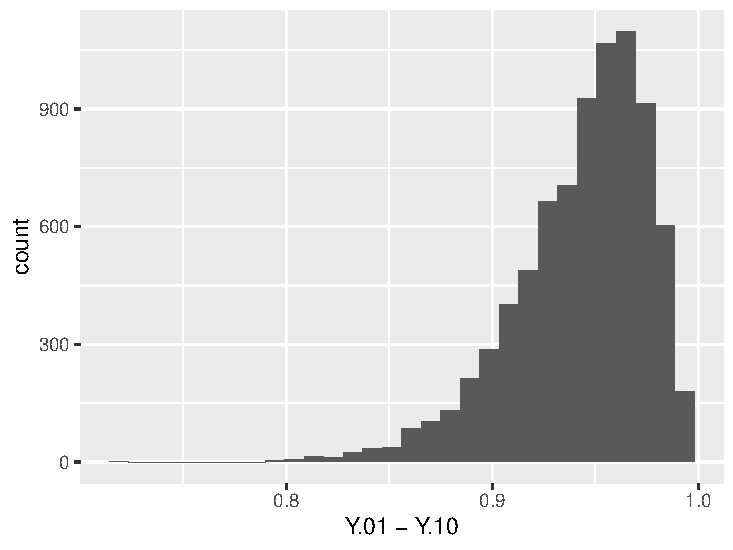
\includegraphics{paper_files/figure-pdf/unnamed-chunk-38-1.pdf}

\hypertarget{query-distribution}{%
\subsection{Query distribution}\label{query-distribution}}

\texttt{query\_distribution} works similarly except that distributions
over queries are returned:

\begin{verbatim}
make_model("X -> Y") |> 
  query_distribution(
    query = list(increasing = "(Y[X=1] > Y[X=0])"), 
    using = "priors") |>
  ggplot(aes(increasing)) +
  geom_histogram()
\end{verbatim}

\begin{verbatim}
`stat_bin()` using `bins = 30`. Pick better value with `binwidth`.
\end{verbatim}

\begin{figure}[H]

{\centering 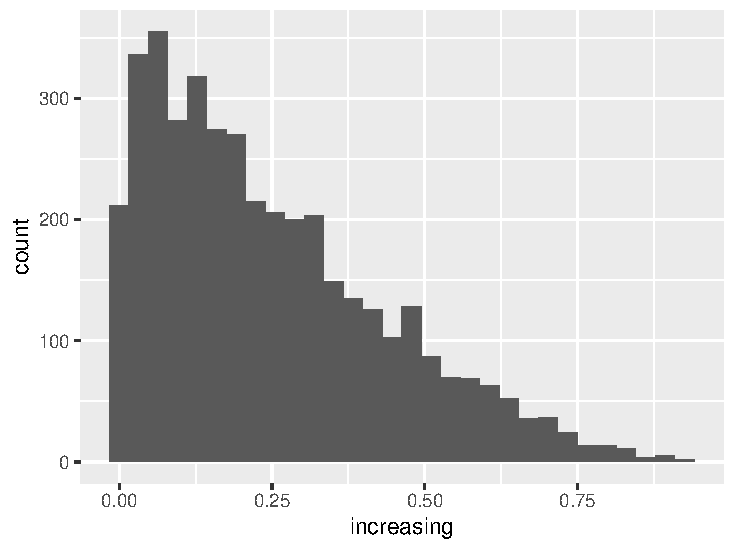
\includegraphics{paper_files/figure-pdf/unnamed-chunk-39-1.pdf}

}

\caption{Prior on 'Probability \(Y\) is increasing in \(X\)'}

\end{figure}

\hypertarget{case-level-queries}{%
\subsection{Case level queries}\label{case-level-queries}}

MH

Case level queries provide the inference for a `new case', which is a
scalar The case level query \emph{updates} on the given information
observed in the new case. The resulting inference is different to the
inference that would be made from the posterior \emph{given} the
features of the case.

To illustrate, consider a model for which we are quite sure that \(X\)
causes \(Y\) but we do not know whether it works through two positive
effects or two negative effects. Thus we do not know if M=0 would
suggest an effect or no effect. If asked what we would infer for a case
that had \(M=0\) we would not know whether \(M=0\) information is
consistent with a positive effect or not. However if provided with a
randomly case and learn that it has \(M=0\), then we update about the
causal model and infer that there is an effect in this case (but that
there wouldn't be were \(M=1\)).

\begin{verbatim}
# DO ALL THIS IN ONE TABLE

set.seed(1)
 model <-
   make_model("X -> M -> Y") |>
   update_model(data.frame(X = rep(0:1, 8), Y = rep(0:1, 8)), iter = 10000)

 Q <- "Y[X=1] > Y[X=0]"
 G <- "X==1 & Y==1 & M==1"
 QG <- "(Y[X=1] > Y[X=0]) & (X==1 & Y==1 & M==1)"

 # In this case these are very different:
 query_distribution(model, Q, given = G, using = "posteriors")[[1]] |> mean()
 query_distribution(model, Q, given = G, using = "posteriors",
   case_level = TRUE)

 # These are equivalent:
 # 1. Case level query via function
 query_distribution(model, Q, given = G,
    using = "posteriors", case_level = TRUE)

 # 2. Case level query by hand using Bayes
 distribution <- query_distribution(
    model, list(QG = QG, G = G), using = "posteriors")

 mean(distribution$QG)/mean(distribution$G)
\end{verbatim}

\hypertarget{batch-queries}{%
\subsection{Batch queries}\label{batch-queries}}

The \texttt{query\_model} function takes causal queries and conditions
(\texttt{given}) and specifies the parameters to be used. The result is
a dataframe which can be displayed as a table.

\begin{verbatim}
models <- list(
 `1` = make_model("X -> Y"),
 `2` = make_model("X -> Y") |> set_restrictions("Y[X=1] < Y[X=0]")
 )

query_model(
  models,
  query = list(ATE = "Y[X=1] - Y[X=0]", POS = "Y[X=1] > Y[X=0]"),
  given = c(TRUE,  "Y==1 & X==1"),
  case_level = c(FALSE, TRUE),
  using = c("parameters", "priors"),
  expand_grid = TRUE) |>
  select(-starts_with("cred")) |>
  
  kable(digits = 2)
\end{verbatim}

\begin{longtable}[]{@{}lllllrr@{}}
\toprule\noalign{}
model & query & given & using & case\_level & mean & sd \\
\midrule\noalign{}
\endhead
\bottomrule\noalign{}
\endlastfoot
1 & ATE & - & parameters & FALSE & 0.00 & NA \\
2 & ATE & - & parameters & FALSE & 0.33 & NA \\
1 & ATE & - & priors & FALSE & 0.00 & 0.32 \\
2 & ATE & - & priors & FALSE & 0.32 & 0.23 \\
1 & ATE & Y==1 \& X==1 & parameters & FALSE & 0.50 & NA \\
2 & ATE & Y==1 \& X==1 & parameters & FALSE & 0.50 & NA \\
1 & ATE & Y==1 \& X==1 & priors & FALSE & 0.51 & 0.29 \\
2 & ATE & Y==1 \& X==1 & priors & FALSE & 0.49 & 0.29 \\
1 & POS & - & parameters & FALSE & 0.25 & NA \\
2 & POS & - & parameters & FALSE & 0.33 & NA \\
1 & POS & - & priors & FALSE & 0.25 & 0.19 \\
2 & POS & - & priors & FALSE & 0.32 & 0.23 \\
1 & POS & Y==1 \& X==1 & parameters & FALSE & 0.50 & NA \\
2 & POS & Y==1 \& X==1 & parameters & FALSE & 0.50 & NA \\
1 & POS & Y==1 \& X==1 & priors & FALSE & 0.51 & 0.29 \\
2 & POS & Y==1 \& X==1 & priors & FALSE & 0.49 & 0.29 \\
1 & ATE & - & parameters & TRUE & 0.00 & NA \\
2 & ATE & - & parameters & TRUE & 0.33 & NA \\
1 & ATE & - & priors & TRUE & 0.00 & NA \\
2 & ATE & - & priors & TRUE & 0.32 & NA \\
1 & ATE & Y==1 \& X==1 & parameters & TRUE & 0.50 & NA \\
2 & ATE & Y==1 \& X==1 & parameters & TRUE & 0.50 & NA \\
1 & ATE & Y==1 \& X==1 & priors & TRUE & 0.50 & NA \\
2 & ATE & Y==1 \& X==1 & priors & TRUE & 0.49 & NA \\
1 & POS & - & parameters & TRUE & 0.25 & NA \\
2 & POS & - & parameters & TRUE & 0.33 & NA \\
1 & POS & - & priors & TRUE & 0.25 & NA \\
2 & POS & - & priors & TRUE & 0.32 & NA \\
1 & POS & Y==1 \& X==1 & parameters & TRUE & 0.50 & NA \\
2 & POS & Y==1 \& X==1 & parameters & TRUE & 0.50 & NA \\
1 & POS & Y==1 \& X==1 & priors & TRUE & 0.50 & NA \\
2 & POS & Y==1 \& X==1 & priors & TRUE & 0.49 & NA \\
\end{longtable}

\hypertarget{computational-details-and-software-requirements}{%
\section*{Computational details and software
requirements}\label{computational-details-and-software-requirements}}
\addcontentsline{toc}{section}{Computational details and software
requirements}

TILL TEXT

\begin{itemize}
\tightlist
\item
  information about certain computational details such as version
  numbers, operating systems, or compilers could be included in an
  unnumbered section. Also, auxiliary packages (say, for visualizations,
  maps, tables, \ldots) that are not cited in the main text can be
  credited here.
\end{itemize}

:::

The results in this paper were obtained using
\proglang{R}\textasciitilde3.4.1 with the
\pkg{MASS}\textasciitilde7.3.47 package. \proglang{R} itself and all
packages used are available from the Comprehensive \proglang{R} Archive
Network (CRAN) at {[}https://CRAN.R-project.org/{]}.

\hypertarget{acknowledgments}{%
\section*{Acknowledgments}\label{acknowledgments}}
\addcontentsline{toc}{section}{Acknowledgments}

\begin{tcolorbox}[enhanced jigsaw, breakable, rightrule=.15mm, leftrule=.75mm, colback=white, bottomrule=.15mm, arc=.35mm, opacityback=0, toprule=.15mm, left=2mm]

The approach to generating a generic stan function that can take data
from arbitrary models was developed in key contributions by
\href{http://jasper-cooper.com/}{Jasper Cooper} and
\href{http://gsyunyaev.com/}{Georgiy Syunyaev}.
\href{https://lilymedina.github.io/}{Lily Medina} did magical work
pulling it all together and developing approaches to characterizing
confounding and defining estimands. Clara Bicalho helped figure out the
syntax for causal statements. Julio Solis made many key contributions
figuring out how to simplify the specification of priors. Merlin
Heidemanns figured out the \texttt{rstantools} integration and made
myriad code improvements. Till Tietz revamped the entire package and
improved every part of it.

\end{tcolorbox}

\hypertarget{references}{%
\section*{References}\label{references}}
\addcontentsline{toc}{section}{References}

\renewcommand{\bibsection}{}
\bibliography{bib.bib}

\newpage{}

\hypertarget{sec-techdetails}{%
\section*{More technical details}\label{sec-techdetails}}
\addcontentsline{toc}{section}{More technical details}

\begin{tcolorbox}[enhanced jigsaw, breakable, rightrule=.15mm, leftrule=.75mm, colback=white, bottomrule=.15mm, arc=.35mm, opacityback=0, toprule=.15mm, left=2mm]

Appendices can be included after the bibliography (with a page break).
Each section within the appendix should have a proper section title
(rather than just \emph{Appendix}).

For more technical style details, please check out JSS's style FAQ at
{[}https://www.jstatsoft.org/pages/view/style\#frequently-asked-questions{]}
which includes the following topics:

\begin{itemize}
\tightlist
\item
  Title vs.~sentence case.
\item
  Graphics formatting.
\item
  Naming conventions.
\item
  Turning JSS manuscripts into \proglang{R} package vignettes.
\item
  Trouble shooting.
\item
  Many other potentially helpful details\ldots{}
\end{itemize}

\end{tcolorbox}

\hypertarget{sec-bibtex}{%
\section*{Using BibTeX}\label{sec-bibtex}}
\addcontentsline{toc}{section}{Using BibTeX}

\begin{tcolorbox}[enhanced jigsaw, breakable, rightrule=.15mm, leftrule=.75mm, colback=white, bottomrule=.15mm, arc=.35mm, opacityback=0, toprule=.15mm, left=2mm]

References need to be provided in a \textsc{Bib}{\TeX} file
(\texttt{.bib}). All references should be made with \texttt{@cite}
syntax. This commands yield different formats of author-year citations
and allow to include additional details (e.g.,pages, chapters, \dots) in
brackets. In case you are not familiar with these commands see the JSS
style FAQ for details.

Cleaning up \textsc{Bib}{\TeX} files is a somewhat tedious task --
especially when acquiring the entries automatically from mixed online
sources. However, it is important that informations are complete and
presented in a consistent style to avoid confusions. JSS requires the
following format.

\begin{itemize}
\tightlist
\item
  item JSS-specific markup (\texttt{\textbackslash{}proglang},
  \texttt{\textbackslash{}pkg}, \texttt{\textbackslash{}code}) should be
  used in the references.
\item
  item Titles should be in title case.
\item
  item Journal titles should not be abbreviated and in title case.
\item
  item DOIs should be included where available.
\item
  item Software should be properly cited as well. For \proglang{R}
  packages \texttt{citation("pkgname")} typically provides a good
  starting point.
\end{itemize}

\end{tcolorbox}

\hypertarget{appendix-stan-code}{%
\section{Appendix: stan code}\label{appendix-stan-code}}

\texttt{prep\_stan\_data} then returns a list of objects that
\texttt{stan} expects to receive. These include indicators to figure out
where a parameter set starts (\texttt{l\_starts}, \texttt{l\_ends}) and
ends and where a data strategy starts and ends
(\texttt{strategy\_starts}, \texttt{strategy\_ends}), as well as the
matrices described above.

MOVE TO APPENDIX? ADD DISCUSSION OF PARMAP

Below we show the \texttt{stan} code. This starts off with a block
saying what input data is to be expected. Then there is a
characterization of parameters and the transformed parameters. Then the
likelihoods and priors are provided. \texttt{stan} takes it from there
and generates a posterior distribution.

\begin{verbatim}
functions{
  row_vector col_sums(matrix X) {
    row_vector[cols(X)] s ;
    s = rep_row_vector(1, rows(X)) * X ;
    return s ;
  }
}
data {
int<lower=1> n_params;
int<lower=1> n_paths;
int<lower=1> n_types;
int<lower=1> n_param_sets;
int<lower=1> n_nodes;
int<lower=1> n_param_each[n_param_sets];
int<lower=1> n_data;
int<lower=1> n_events;
int<lower=1> n_strategies;
int<lower=0, upper=1> keep_transformed;
vector<lower=0>[n_params] lambdas_prior;
int<lower=1> l_starts[n_param_sets];
int<lower=1> l_ends[n_param_sets];
int<lower=1> node_starts[n_nodes];
int<lower=1> node_ends[n_nodes];
int<lower=1> strategy_starts[n_strategies];
int<lower=1> strategy_ends[n_strategies];
matrix[n_params, n_types] P;
matrix[n_params, n_paths] parmap;
matrix[n_paths, n_data] map;
matrix<lower=0,upper=1>[n_events,n_data] E;
int<lower=0> Y[n_events];
}
parameters {
vector<lower=0>[n_params - n_param_sets] gamma;
}
transformed parameters {
vector<lower=0>[n_params] lambdas;
vector<lower=1>[n_param_sets] sum_gammas;
matrix[n_params, n_paths] parlam;
matrix[n_nodes, n_paths] parlam2;
vector<lower=0, upper=1>[n_paths] w_0;
vector<lower=0, upper=1>[n_data] w;
vector[n_events] w_full;
// Cases in which a parameter set has only one value need special handling
// they have no gamma components and sum_gamma needs to be made manually
for (i in 1:n_param_sets) {
if (l_starts[i] >= l_ends[i]) {
  sum_gammas[i] = 1;
  // syntax here to return unity as a vector
  lambdas[l_starts[i]] = lambdas_prior[1]/lambdas_prior[1];
  }
else if (l_starts[i] < l_ends[i]) {
  sum_gammas[i] =
  1 + sum(gamma[(l_starts[i] - (i-1)):(l_ends[i] - i)]);
  lambdas[l_starts[i]:l_ends[i]] =
  append_row(1, gamma[(l_starts[i] - (i-1)):(l_ends[i] - i)]) / sum_gammas[i];
  }
  }
// Mapping from parameters to data types
parlam  = rep_matrix(lambdas, n_paths) .* parmap; // (usual case): [n_par * n_data] * [n_par * n_data]
// Sum probability over nodes on each path
for (i in 1:n_nodes) {
 parlam2[i,] = col_sums(parlam[(node_starts[i]):(node_ends[i]),]);
 }
// then take product  to get probability of data type on path
for (i in 1:n_paths) {
  w_0[i] = prod(parlam2[,i]);
 }
 // last (if confounding): map to n_data columns instead of n_paths
 w = map'*w_0;
 w = w / sum(w);
 w_full = E * w;
}
model {
// Dirichlet distributions (earlier versions used gamma)
for (i in 1:n_param_sets) {
  target += dirichlet_lpdf(lambdas[l_starts[i]:l_ends[i]]  | lambdas_prior[l_starts[i] :l_ends[i]]);
  target += -n_param_each[i] * log(sum_gammas[i]);
 }
// Multinomials
for (i in 1:n_strategies) {
  target += multinomial_lpmf(
  Y[strategy_starts[i]:strategy_ends[i]] | w_full[strategy_starts[i]:strategy_ends[i]]);
 }
}
// Option to export distribution of causal types
// Note if clause used here to effectively turn off this block if not required
generated quantities{
vector[n_types] prob_of_types;
if (keep_transformed == 1){
for (i in 1:n_types) {
   prob_of_types[i] = prod(P[, i].*lambdas + 1 - P[,i]);
}}
 if (keep_transformed == 0){
    prob_of_types = rep_vector(1, n_types);
 }
}
\end{verbatim}




\end{document}
